\chapter{Evaluierung der Verwendbarkeit des Werkzeugs} % (fold)
\label{cha:eval_werkzeug}

Im ersten empirischen Teil der Evaluierung wurde die grundlegende Verständlichkeit und Verwendbarkeit des Werkzeug geprüft. Ziel war es hier, konzeptionelle und technische Eigenschaften bzw. Verhaltensweisen des Werkzeugs zu identifizieren, die den Modellierungsprozess behindern oder unterbrechen. Darunter fällt grundsätzlich jede Eigenschaft und jede Verhaltensweise, die die Benutzer zwingt, sich mit dem technischen System an sich zu beschäftigen und von der Erfüllung der eigentlichen Aufgabe ablenkt bzw. diese unterbricht. Abbildung \ref{fig:img_Kontextgrafiken_k12} stellt dieses Kapitel und dessen Aufbau im Kontext der anderen inhaltlich vor- und nachgelagerten Kapitel dar.

\begin{figure}[htbp]
	\centering
		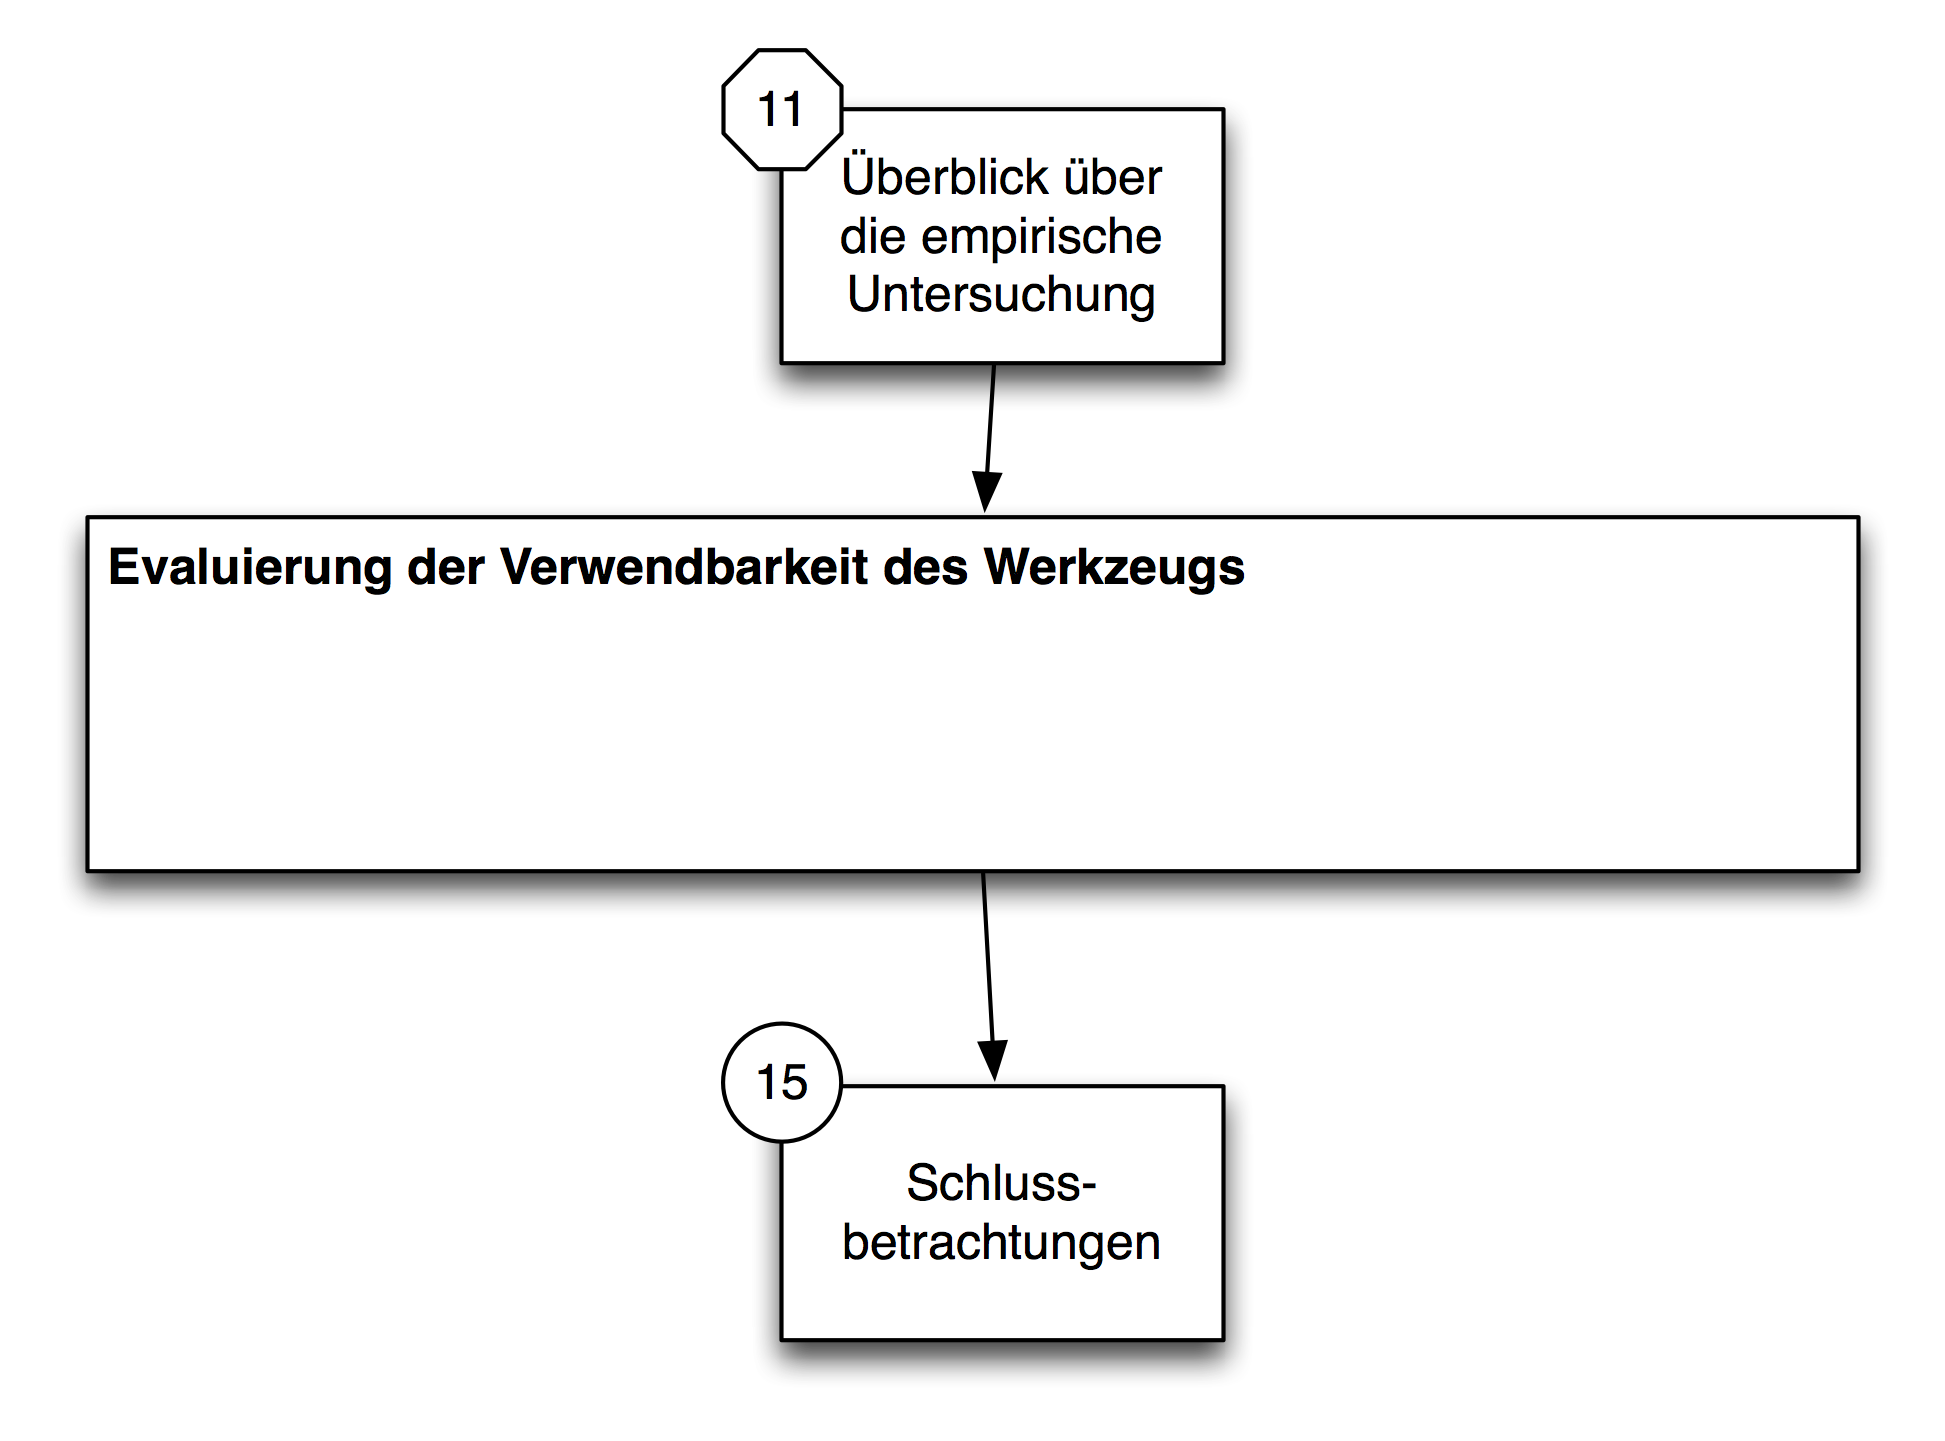
\includegraphics[scale=0.6]{img/Kontextgrafiken/k12.png}
	\caption{Kapitel „Evaluierung der Verwendbarkeit des Werkzeugs“ im Gesamtzusammenhang}
	\label{fig:img_Kontextgrafiken_k12}
\end{figure}

Die Untersuchung wurde daneben auch genutzt, um explorativ die inhaltliche Verwendung des Systems zu untersuchen (d.h. wie es für seinen eigentlichen Verwendungszweck, die Modellierung, eingesetzt wurde) und Hypothesen abzuleiten, die in weiteren Schritten getestet werden konnten.

\section{Hypothesen} % (fold)
\label{sec:hypothesen}

In diesem Abschnitt werden die Hypothesen angeführt und begründet, die in diesem Teil der empirischen Untersuchung geprüft werden. Die hier angegebenen Hypothesen gehen auf die Eigenschaften des Werkzeugs in der Verwendung durch die Benutzer ein. Bei der Hypothesenbildung wird auf den Verwendungszweck des Werkzeugs, die Unterstützung der Bildung diagrammatischer Modelle, Rücksicht genommen -- die Modelle selbst sind jedoch nicht Gegenstand der Betrachtung, sondern werden erst im nächsten Kapitel behandelt. Nicht berücksichtigt wird außerdem die Verwendung zur Unterstützung von Articulation Work -- die Implikationen des Werkzeugs auf diese sind Gegenstand von Kapitel \ref{cha:eval_aw}.

\subsection{Konzeptionell begründete Hypothesen} % (fold)
\label{sub:konzeptionell_begründete_hypothesen}

Die folgenden Hypothesen wurden aus der Aufgabenstellung (siehe Kapitel \ref{cha:einführung}) sowie den Anforderungen an das Werkzeug (siehe Kapitel \ref{cha:anforderungen}) abgeleitet. Neben der Formulierung der Hypothese ist jeweils die Begründung aus der Konzeption des Werkzeugs angeführt.

Der grundlegende Anspruch des Werkzeugs ist es, explizite Articulation Work zu unterstützen. Wie in Teil \ref{prt:grundlagen} dieser Arbeit beschrieben, wird dies hier über die Externalisierung und Aushandlung von mentalen Modellen realisiert. Ein gängiges Mittel, um mentale Modelle zu repräsentieren, sind diagrammatische Modelle, worunter die Ergebnisse der vorgeschlagenen Methoden zur Externalisierung -- Concept Mapping und Strukturlegetechniken -- fallen. Das Werkzeug muss also die Repräsentation diagrammatischer Modelle unterstützen. Die Prüfung dieser Hypothese ermöglicht die Beurteilung der Erfüllung der Anforderung \ref{anf:physische_abbildung_legen_beliebiger_diagrammatischer_modelle} (siehe Seite \pageref{anf:physische_abbildung_legen_beliebiger_diagrammatischer_modelle}). 

\begin{hyp}
	\label{hyp:diagmodelle}
	Das Werkzeug ermöglicht die Repräsentation diagrammatische Modelle.
\end{hyp}

„Articulation Work“ ist immer in einen kooperativen Arbeitszusammenhang eingebettet. Die Kollaboration findet dabei nicht nur im produktiven Teil der Arbeit statt, sondern hat immer auch Auswirkungen auf die „Articulation Work“. Jede Unterstützung von „Articulation Work“ muss damit auch in kooperativen Szenarien einsetzbar sein. Dies gilt auch für das hier vorgestellte Werkzeug, das die kooperative Bearbeitung einer Aufgaben (hier: der Externalisierung und Abstimmung mentaler Modelle) ermöglichen muss. Die Prüfung dieser Hypothese ermöglicht die Beurteilung der Erfüllung der Anforderung \ref{anf:kollaborative_und_unmittelbare_manipulierbarkeit_des_modells} (siehe Seite \pageref{anf:kollaborative_und_unmittelbare_manipulierbarkeit_des_modells}).

\begin{hyp}
	\label{hyp:kollaborativ}
	Das Werkzeug ermöglicht kooperatives Arbeiten an einer Aufgabe.
\end{hyp}

Die Aspekte von Arbeit, die im Rahmen von „Articulation Work“ abzustimmen sind, sind unterschiedlicher Natur. Naheliegend ist eine Abstimmung der Abläufe und Schnittstellen zwischen Personen, aber auch nicht-prozedurale Information wie das Verständnis der Struktur und Elemente eines Arbeitszusammenhangs kann Gegenstand von Articulation Work sein. Gleiches gilt für die im Rahmen der Articulation Work abzustimmenden mentalen Modelle -- diese bilden die Basis für Handlungsentscheidungen, umfassen aber im Allgemeinen (in Abgrenzung zu Schemata) nicht nur handlungsleitende Information sondern auch Kontextinformation, die die Bewertung der wahrgenommenen Situation ermöglicht. Demensprechend muss ein Werkzeug zu Unterstützung von expliziter Articulation Work und damit der Externalisierung von mentalen Modellen die Verwendung in unterschiedlichen Kontexten, d.h. für unterschiedliche zu externalisierenden Informationsstrukturen, die in mentalen Modellen abgebildet sind, ermöglichen. Die Prüfung dieser Hypothese ermöglicht die Beurteilung der Erfüllung der Anforderung \ref{anf:nicht_vorgegebene_semantik_der_modellierungselemente} (siehe Seite \pageref{anf:nicht_vorgegebene_semantik_der_modellierungselemente}).

\begin{hyp}
	\label{hyp:kontexte}
	Das Werkzeug ist gleichwertig für Modellierungsaufgaben in unterschiedlichen Kontexten einsetzbar.
\end{hyp}

Die ersten drei hier formulierten Hypothesen sind unmittelbar aus der globalen Zielsetzung abgeleitet und bilden die grundlegenden Anforderungen an das Werkzeug bei der Unterstützung von Articulation Work ab. Die nun folgenden Hypothesen sind konzeptionell nicht mehr direkt auf die globale Zielsetzung ausgerichtet sondern stellen auf Funktionalität des Werkzeugs ab, die den Modellbildungsprozess unterstützen soll. 

Auf Basis der Möglichkeit zur Navigation durch die Entstehungsgeschichte des Modells besteht auch die Möglichkeit, vergangene Modellzustände wiederherzustellen. Das Werkzeug unterstützt dabei die Benutzer durch die Ausgabe von schrittweisen Anweisungen, die den aktuellen Modellzustand in den wiederherzustellenden Zustand überführen. Allgemein bietet diese Funktionalität die Möglichkeit, erkannte Fehler im Modell zu korrigieren, ohne dabei bereits repräsentierte Information zu verlieren. Im kollaborativen Einsatz ermöglicht diese Funktionalität, alternative, individuelle Sichten auf den abzustimmenden Sachverhalt zu repräsentieren und dabei die Möglichkeit bieten, einen für alle Beteiligten akzeptablen Ausgangspunkt wiederherzustellen. Die Prüfung dieser Hypothese ermöglicht die Beurteilung der Erfüllung der Anforderung \ref{anf:ermöglichung_experimenteller_veränderungen_am_modell} (siehe Seite \pageref{anf:ermöglichung_experimenteller_veränderungen_am_modell}).

\begin{hyp}
	\label{hyp:wiederherstellung}
	Die Möglichkeit der Wiederherstellung vergangener Modellzustände fördert die Bereitschaft alternative Repräsentationen auszuprobieren.
\end{hyp}

Die letzten beiden Hypothesen dieses Abschnitts sind ausschließlich auf die Verwendung des Werkzeugs an sich ausgerichtet und stehen nicht im Kontext von Articulation Work oder der Unterstützung der Externalisierung mentaler Modelle. Hypothese \ref{hyp:behinderung} steht für den in der Zielsetzung formulierten Anspruch, dass das Werkzeug in den Hintergrund treten muss und die Beschäftigung mit der eigentlichen Aufgabe nicht behindern darf. Dabei wird hier nicht auf den konkreten Anwendungsfall -- die Erstellung von Modellen -- eingegangen sondern lediglich die allgemeine Funktionsfähigkeit und Bedienbarkeit des Werkzeugs betrachtet. Ersteres ist Gegenstand der Evaluierung der erstellten Modelle, die in Kapitel \ref{cha:eval_modell} beschrieben werden. Die Prüfung dieser Hypothese ermöglicht die Beurteilung der Erfüllung der Anforderung \ref{anf:physische_abbildung_legen_beliebiger_diagrammatischer_modelle} (siehe Seite \pageref{anf:physische_abbildung_legen_beliebiger_diagrammatischer_modelle}).

\begin{hyp}
	\label{hyp:behinderung}
	Das Werkzeug behindert die Modellbildung nicht.
\end{hyp}

Hypothese \ref{hyp:gewöhnung} geht davon aus, dass bei wiederholten Verwendung des Werkzeugs Lern- und Gewöhnungseffekte auftreten, die die Verwendung erleichtern, beschleunigen und zu weniger Fehlbedienung führen. Dies ist ein Effekt, der bei jedem Werkzeug zu erwarten ist, dessen zugrunde liegenden Konzepte den Benutzern bewusst sind. Von dieser Voraussetzung kann durch die inhaltliche Einführung der Benutzer in die das Werkzeug prägenden und motivierenden Ideen ausgegangen werden. Damit wäre zu erwarten, dass das Werkzeug bei wiederholtem Einsatz in den späteren Anwendungen effizienter (im Sinne von schneller und Fehlbedienungen vermeidend) verwendet wird. Die Prüfung dieser Hypothese ermöglicht die Beurteilung der Erfüllung der Anforderung \ref{anf:physische_abbildung_legen_beliebiger_diagrammatischer_modelle} (siehe Seite \pageref{anf:physische_abbildung_legen_beliebiger_diagrammatischer_modelle}).

\begin{hyp}
	\label{hyp:gewöhnung}
	Wiederholte Verwendung des Werkzeugs führt zu schnellerer Modellbildung und weniger Fehlbedienungen.
\end{hyp}

Hinsichtlich der in Kapitel \ref{cha:anforderungen} formulierten Anforderungen können die hier formulierten Hypothesen zusammenfassend wie in Tabelle \ref{hyp:eval_tui} dargestellt eingeordnet werden:

\begin{table}[htbp]
	\centering
	\caption{Hypothesen zur Werkzeugbenutzung und deren Bezug zu den Anforderungen an das Werkzeug}
\begin{tabular}{|c|c|}
  \hline
   Hypothese & Anforderung \\ \hline
   \ref{hyp:diagmodelle} & \ref{anf:physische_abbildung_legen_beliebiger_diagrammatischer_modelle} \\
   \ref{hyp:kollaborativ} & \ref{anf:kollaborative_und_unmittelbare_manipulierbarkeit_des_modells} \\
   \ref{hyp:kontexte} & \ref{anf:nicht_vorgegebene_semantik_der_modellierungselemente} \\
   \ref{hyp:wiederherstellung} & \ref{anf:ermöglichung_experimenteller_veränderungen_am_modell} \\
   \ref{hyp:behinderung} & \ref{anf:physische_abbildung_legen_beliebiger_diagrammatischer_modelle} \\
   \ref{hyp:gewöhnung} & \ref{anf:physische_abbildung_legen_beliebiger_diagrammatischer_modelle} \\ \hline
\end{tabular} 
	\label{hyp:eval_tui}
\end{table}

% subsection konzeptionell_begründete_hypothesen (end)

\subsection{Explorativ gebildete Hypothesen} % (fold)
\label{sub:explorativ_gebildete_hypothesen}

Neben den aus der Aufgabenstellung abgeleiteten Hypothesen wurden einige Hypothesen auch während der Durchführung der einzelnen Evaluierungs-Blöcke gebildet. Diese Hypothesen sind spezifischer auf einzelne Aspekte des Werkzeugs abgestellt und decken beobachtete Auffälligkeiten und Missverständnisse in der Verwendung des Werkzeugs ab. 

Die erste in diesem Zusammenhang beobachtete Auffälligkeit betrifft die Herstellung von Verbindern zwischen einzelnen Modellelementen. Wie in Abschnitt \ref{sub:verbinden_von_modellelementen} beschrieben, existieren zwei Möglichkeiten, diese Funktion auszuführen. Einerseits können die beiden Modellelemente, die verbunden werden sollen, mit Markierungs-Tokens ausgewählt werden, worauf hin eine Verbindung hergestellt werden. Andererseits können Verbinder auch durch das Zusammenführen der zu verbindenden Blöcke (bis sich deren Breitseiten berühren) hergestellt werden. In der ersten Implementierung des Werkzeugs, die im Evaluierungs-Block 1 und im ersten Teil des zweiten Blocks verwendet wurde, war lediglich die erste Variante verfügbar. Die Möglichkeit zur Herstellung von Verbindern wurde in den in diesen Blöcken durchgeführten Anwendungen kaum eingesetzt. Dies führte einerseits zur Bildung der Hypothese \ref{hyp:keine_verbinder} (siehe Abschnitt \ref{sub:m_explorativ_gebildete_hypothesen}), andererseits wurde bei ersten Auswertungen der Beobachtungen der im Verhältnis zum übrigen Modellierungs-Prozess hohe Zeit-Aufwand bei der Herstellung von Verbindern offensichtlich. Dieser Aufwand ist den Maßnahmen zur Stabilisierung der Erkennungsleistung des Werkzeugs geschuldet und kann mit den eingesetzten Interaktionsablauf nicht reduziert werden. Aufgrund einer Anregung eines Untersuchungsteilnehmers wurde deshalb die oben beschriebene zusätzliche Möglichkeit zur Herstellung von Verbindungen implementiert. Zu untersuchen ist nun, ob diese Maßnahme die Nutzung von Verbindern bei der Modellbildung tatsächlich erhöht.

\begin{hyp}
	\label{hyp:verbinder}
	Die Einführung der alternativen Möglichkeit zur Verbindungsherstellung erhöht die Nutzung von Verbindern bei der Modellerstellung.
\end{hyp}

Die zweite hier aufgestellte Hypothese betrifft eine Auffälligkeit bei der Verwendung des Löschtokens. Das Löschtoken wird verwendet, um das Werkzeug in einen Modus zu versetzen, in dem Verbinder gelöscht werden können. Schon die konzeptionelle Einordnung des Werkzeugs in Kapitel \ref{cha:konzeptionelle_evaluierung} zeigte Potential für Missverständnisse in der Verwendung dieses Tokens (siehe z.B. die Abschnitte \ref{sec:spezifikation_des_tac_schemas_nach_shaer_et_al_} und \ref{sec:einordnung_in_die_taxonomie_von_fishkin}). Zusammengefasst liegt die aus der Theorie ableitbare Problematik darin, dass durch die äußere Form des Tokens -- einem Radiergummi -- eine Metapher für dessen Verwendung („ausradieren“ von Elementen) suggeriert wird, die in dieser Form im Werkzeug nicht umgesetzt ist, da das Token lediglich als Schalter fungiert. Erste Beobachtungen deuteten darauf hin, dass die Verwendung des Löschtoken tatsächlich unverständlich oder missverständlich zu sein scheint. Die zugehörige Hypothese ist positiv formuliert, zu erwarten wäre demnach, dass sie verworfen werden muss.

\begin{hyp}
	\label{hyp:radierer}
	Das Löschtoken ermöglicht intuitives Löschen von Modellelementen.
\end{hyp}

% subsection explorativ_gebildete_hypothesen (end)
% section hypothesen (end)

\section{Untersuchungsdesign und Durchführung} % (fold)
\label{sec:untersuchungsdesign}

In diesem Abschnitt wird auf Basis der oben formulierten Hypothesen das Untersuchungsdesign abgeleitet und die Durchführung der Untersuchung beschrieben. Der erste Teil des Abschnitts beschreibt die Operationalisierung der Hypothesen und damit die Festlegung wie diese konkret geprüft werden können. Im zweiten Teil des Abschnitts wird die Durchführung der Prüfung beschrieben. Hier erfolgt neben der Zuordnung der einzelnen Evaluierungsblöcke (siehe Abschnitt \ref{sec:globales_untersuchungsdesign}) auch die Darstellung rein beschreibender Parameter der Werkzeugverwendung, die nicht unmittelbar in die Prüfung der Hypothesen eingehen. 

\subsection{Operationalisierung} % (fold)
\label{sub:operationalisierung}

In diesem Abschnitt wird für jede Hypothese identifiziert, in welcher Form sie geprüft werden kann. Dies umfasst die Festlegung der Messpunkte sowie der jeweiligen Mess- und Auswertungsmethode (letzte bezugnehmend auf den in Abschnitt \ref{sec:eingesetzte_werkzeuge_und_verfahren} beschriebenen Verfahren). Zudem werden jene Evaluationsblöcke festgelegt, die für die jeweilige Untersuchung herangezogen wurden.

Für jede Hypothese wird also spezifiziert, anhand welcher Aspekte diese geprüft werden kann (= abhängige Variablen). Zudem wird festgelegt welche Ausgangssituation bei der Anwendung gewählt werden muss, um die Prüfung durchführen zu können (= unabhängige Variable) und welche Faktoren die Beurteilung ggf. ungewollt beeinflussen können (= Störvariablen).

\subsubsection{Repräsentation diagrammatischer Modelle} % (fold)
\label{ssub:repräsentation}

Gegenstand dieses Abschnitts ist die Prüfung der Hypothese \ref{hyp:diagmodelle}. Diese bezieht sich auf die Eignung des Werkzeugs für die Repräsentation diagrammatischer Modelle.

Voraussetzung für die Prüfung der Hypothese ist der Einsatz von Modellierungsaufgaben, die so formuliert sind, dass es grundsätzlich möglich ist, sie durch die Beschreibung in einem diagrammatischen Modell zu erfüllen. Keinen Einfluss auf die Untersuchung haben die eingesetzte Methodik sowie eventuell vorhandene Modellierungsvorkenntnisse, da die grundsätzlich Möglichkeit der Erstellung diagrammatischer Modelle unabhängig von der Art der Verwendung und von der Kompetenz der Benutzer ist. 

Geprüft wird die Hypothese hier an der Repräsentation, die mit Hilfe des Werkzeugs erstellt wurde. Ein diagrammatisches Modell zeichnet nach \citep{Larkin87} aus, dass in ihm Konzepte und deren Zusammenhänge visuell-graphisch dargestellt werden können (in Abgrenzung zu textuellen Beschreibungen). Zur Bewertung der Hypothese werden deshalb die erstellten Repräsentationen herangezogen und überprüft, ob sie den Anforderungen an ein diagrammatisches Modell -- das Vorhandensein von Konzepten und Beziehungen zwischen diesen -- erfüllen.

% subsubsection repräsentation (end)

\subsubsection{Kooperatives Arbeiten} % (fold)
\label{ssub:kollaboratives_arbeiten}

Gegenstand dieses Abschnitts ist die Prüfung der Hypothese \ref{hyp:kollaborativ}. Dabei wird überprüft, ob das Werkzeug kooperatives Arbeiten an einer Modellierungsaufgabe erlaubt.

Dazu muss eine Modellierungsaufgabe gewählt werden, in der die kooperatives Erstellung des Modells vorgesehen ist. Etwaige Modellierungsvorkenntnisse haben keinen Einfluss auf die Beurteilung der hier betrachteten Hypothese.

Zur Beurteilung eignen sich in diesem Fall die Zeitverteilung der Beteiligung der einzelnen Benutzer am Modellierungsvorgang, das Verhalten der Benutzer bei simultaner Manipulation eines Modells auf der Modellierungsoberfläche sowie der subjektive Eindruck der Benutzer über deren Kooperation untereinander. Der erstgenannte Aspekt kann quantitativ gemessen werden, wobei eine tendenziell zeitlich gleichverteilte Einbindung der Beteiligten in die Modellbildung für die Annahme der Hypothese spricht. Zusätzlich kann mittels dem zweiten und dritten Aspekt qualitativ beurteilt werden, ob und wie eine kooperative Manipulation des Modells durch mehrere Benutzer gleichzeitig möglich ist.

% subsubsection kollaboratives_arbeiten (end)

\subsubsection{Einsetzbarkeit in unterschiedlichen Kontexten} % (fold)
\label{ssub:einsetzbarkeit_in_unterschiedlichen_kontexten}

Gegenstand dieses Abschnitts ist die Operationalisierung der Hypothese \ref{hyp:kontexte}. Diese Hypothese zielt dabei auf die Eignung des Werkzeugs zur Modellbildung in unterschiedlichen Kontexten, d.h. für unterschiedliche Modellierungsaufgaben. 

Zur Beurteilung dieser Hypothese muss die Modellierungsaufgabe entsprechend den unterschiedlichen Einsatzkontexten variiert werden. Etwaige Modellierungsvorkenntnisse können die individuelle Beurteilung insofern beeinflussen, als das sie Werkzeugs für eine bestimmte Aufgabe als besser oder schlechter geeignet erscheinen lassen.

Zur Prüfung der Hypothese bieten sich sind in diesem Fall die Wahrnehmung der Eignung durch die Benutzer, die qualitativ beurteilt wird, und die Korrelation der Größe der erstellten Modelle mit der benötigten Modellierungsdauer an. Korrelliert die Modellgröße positiv mit der Modellierungsdauer, so ist der Zeitanteil, der zu Beschäftigung mit dem Werkzeug selbst (und nicht mit der Modellierungsaufgabe) tendenziell stabil. Daraus kann abgeleitet werden, dass das Werkzeug die verglichenen Modellierungsaufgaben gleich gut (oder schlecht) unterstützt.

% subsubsection einsetzbarkeit_in_unterschiedlichen_kontexten (end)

\subsubsection{Wiederherstellung vergangener Modellzustände} % (fold)
\label{ssub:wiederherstellung_vergangener_modellzustände}

Gegenstand dieses Abschnitts ist die Operationalisierung der Hypothese \ref{hyp:wiederherstellung}. Gegenstand der Überprüfung ist die Verwendung der Wiederherstellungsfunktionalität zum Zwecke der versuchsweisen Veränderung des Modells.

Zur Prüfung dieser Hypothese muss die Modellierungsaufgabe so gestaltet, dass sinnvoll unterschiedliche Repräsentationen gebildet werden können. Modellierungsvorkenntnisse haben keine Auswirkungen auf diese Untersuchung.

Zur Beurteilung dieser Hypothese wird ist die \emph{Anzahl der Verwendungen der Wiederherstellungsfunktionalität zur Korrektur inhaltlich verworfener Repräsentationen} herangezogen. Werte über 0 deuten hier auf eine Annahme der Hypothese hin. Zusätzlich können qualitative Aussagen zur Nutzung dieser Funktionalität und deren \emph{wahrgenommenen Nutzen} zur Beurteilung verwendet werden. 

% subsubsection wiederherstellung_vergangener_modellzustände (end)

\subsubsection{Nicht-Behinderung} % (fold)
\label{ssub:nicht_behinderung}

Gegenstand dieses Abschnitts ist die Operationalisierung der Hypothese \ref{hyp:behinderung}. Dabei wird überprüft, ob bei der Verwendung des Werkzeugs dieses in den Aufmerksamkeitsfokus der Benutzer tritt oder sich diese auf die eigentliche Modellierungsaufgabe konzentrieren können. 

Die Modellierungsaufgabe hat keinen Einfluss auf die Überprüfung dieser Hypothese, lediglich etwaig vorhandene \emph{Modellierungsvorkenntnisse} können als \textbf{Störvariable} wirken, da sie Einfluss auf die erwartete Funktionalität des Werkzeugs haben kann.

Zur Beurteilung, ob bzw. inwieweit das Werkzeug die Modellbildung behindert, werden sowohl quantitativ als auch qualitative beurteilbare Metriken herangezogen. Die Anzahl von \emph{Fehlfunktionen des Werkzeugs} bzw. das \emph{Auftreten von Systemabstürzen} kann als Indikator für eine behindernde Wirkung des Werkzeugs herangezogen werden. Das Auftreten von Missverständnissen und daraus resultierende Fehlbedienungen können ebenfalls eine Behinderung des Modellierungsvorgangs interpretiert werden. Zudem werden Aussagen der Benutzer hinsichtlich hinderlicher Faktoren bei der Werkzeugbenutzung als Maß für die wahrgenommene Behinderung durch das Werkzeug herangezogen. Der Einfluss von Modellierungsvorkenntnissen kann in diesem Fall nicht mit statistischen Maßnahmen kompensiert werden. Etwaige Vorkenntnisse werden dementsprechend bei der Auswertung angeführt und müssen bei der Diskussion der Hypothese berücksichtigt werden.

% subsubsection nicht_behinderung (end)

\subsubsection{Gewöhnung an das Werkzeug} % (fold)
\label{ssub:gewöhnung_an_das_werkzeug}

Gegenstand dieses Abschnitts ist die Operationalisierung der Hypothese \ref{hyp:gewöhnung}. Dabei wird überprüft, ob wiederholte Benutzung des Werkzeugs Auswirkung auf die Qualität der Interaktion hat. Eine Erhöhung der Qualität äußert sich in schnellerer Modellbildung und weniger Fehlbedienung.

Bei der Prüfung der Hypothese muss eine etwaige veränderte Funktionalität des Werkzeugs zwischen den verglichenen Evaluierungsblöcken berücksichtigt werden, die die Interaktion einerseits erleichtern kann, andererseits aber auch zu Fehlbedienung aufgrund von unbekannten Interaktionsmustern führen kann. Auch unterschiedliche Modellierungsaufgaben, die ein Individuum in den aufeinander folgenden Anwendungen bearbeitet, können die Beurteilung erschweren, weil potentiell andere (noch unbekannte) Funktionen des Werkzeugs zum Einsatz kommen können.

Zur Beurteilung der Qualität der Interaktion sind einerseits die Anzahl der Fehlbedienungen des Werkzeugs pro Zeiteinheit und andererseits die Arbeitsdauer am Werkzeug\footnote{Die Arbeitsdauer am Werkzeug ist im Gegensatz zur gesamten Modellierungsdauer um jenen Zeitanteil reduziert, in dem die Teilnehmer interagieren, ohne am Werkzeug zu arbeiten.} in Abhängigkeit der Modellgröße heranzuziehen. Die Normierung der Arbeitsdauer ist notwendig, um vergleichbare Werte für unterschiedliche Werkzeug-Anwendungen zu erhalten. Sinken beide Werte zwischen zwei Evaluierungsblöcken, die auf der gleichen Stichprobe aufbauen, signifikant, so kann die Hypothese bestätigt werden. Um eine Vergleichbarkeit zwischen den Anwendungen herzustellen, ist es sinnvoll, in beiden Blöcken eine identische Modellierungsaufgabe zu stellen und die Funktionalität des Werkzeugs nicht zu verändern. Identische Modellierungsaufgaben können durch die wiederholte inhaltliche Beschäftigung mit der Aufgabe zu schnellerer Arbeit bzw. zu kompakteren Modellen führen. Dies kann wiederum durch die Berücksichtigung der reinen Arbeitszeit am Werkzeug sowie der Normierung derselben in Abhängigkeit der Modellgröße kompensiert werden.

% subsubsection gewöhnung_an_das_werkzeug (end)

\subsubsection{Herstellung von Verbindern} % (fold)
\label{ssub:herstellung_von_verbindern}

Gegenstand dieses Abschnitts ist die Operationalisierung der Hypothese \ref{hyp:verbinder}. Mit Hilfe dieser Hyothese soll überprüft werden, ob die Einführung der alternativen Möglichkeit zur Herstellung von Verbindern deren Verwendung signifikant gesteigert hat.

Bei der Messung muss der Einfluss der Modellierungsaufgabe (da sie die Anzahl der benötigten Verbinder beeinflussen kann) und eventuell vorhandene Modellierungsvorkenntnisse (da diese Einfluss auf die Struktur des Modells haben können) berücksichtigt werden. Um den Einfluss dieser Aspekte zu reduzieren, wird die Beurteilung in zwei Evaluierungsblöcken vorgenommen, in denen die gleiche Stichprobe mit der gleichen Aufgabenstellung das Werkzeug mit der gleichen Methodik anwandte. Lediglich die Funktionalität des Werkzeugs wurde zwischen den beiden Anwendungen um den alternativen Weg zur Herstellung von Verbindern erweitert.  

Zur Beurteilung des Ausmaßes der Verwendung von Verbindern kann die \emph{Connectedness} des Modells herangezogen werden. Die Connectedness ist das Verhältnis zwischen der Anzahl der im Modell verwendeten Verbinder und der Anzahl der verwendeten Knoten (Modellierungselemente). Hier ist zu prüfen, ob die Connectedness in jenem Evaluierungs-Block, in dem der alternative Weg zur Herstellung von Verbindungen verfügbar war, signifikant höher ist als in jenem Block, in dem sie nicht verfügbar war.

% subsubsection herstellung_von_verbindern (end)

\subsubsection{Verwendung des Löschtokens} % (fold)
\label{ssub:löschtoken}

Gegenstand dieses Abschnitts ist die Operationalisierung der Hypothese \ref{hyp:radierer}. Dabei wird überprüft, ob das Löschtoken intuitiv korrekt verwendet wird oder ob es zu Fehlinterpretationen kommt.

Die Verwendbarkeit des Löschtokens ist unabhängig von der Modellierungsaufgabe, der angewandten Methodik und auch von eventuell vorhandenen Modellierungsvorkenntnissen. Hinsichtlich des Anwendungskontext des Werkzeugs sind also keine Voraussetzungen zu beachten.

Zur Beurteilung der intuitiven Verwendbarkeit werden quantitative und qualitative Merkmale der Werkzeugverwendung herangezogen. Quantitativ beurteilbar ist der Anteil der Fehlbedienungen des Löschtokens in Bezug auf alle Anwendungen des Werkzeugs, in denen es grundsätzlich verwendet wurde. Qualitativ wird die Art des Missverständnisses, das zu den jeweiligen Fehlbedienungen führt, beurteilt.

Zur Messung der quantitativen Variablen wird für jede Anwendung die Anzahl der Fehlbedienungen erhoben, die durch das Löschtoken verursacht wurden. Diese Anzahl wird ins Verhältnis zur Gesamtzahl der Anwendungen des Löschtokens bzw. zur gesamten Anzahl der Löschvorgänge gesetzt. Zu letzterer zählen neben den Anwendungen des Löschtokens auch Fehlerkorrekturen durch Verwendung der Wiederherstellungsfunkion. Da die zweite Möglichkeit sowohl zeit- als auch ressourcenaufwändiger zu verwenden ist als der Einsatz der Löschtokens deutet ein hoher Anteil der Verwendung dieser Funktion auf funktionale Probleme oder Verständnisprobleme der eigentlichen Löschfunktion mittels dem Löschtoken hin.  

Qualitativ werden Modellierungssituationen betrachtet, in denen das Löschtoken zum Einsatz kommt. Auf Basis von Transkripten der Interaktion zwischen den Benutzern und dem Werkzeug, bei denen es zu Fehlbedierungen kam, werden die aufgetretenen Missverständnisse explizit identifziert.

% subsubsection löschtoken (end)

% subsection operationalisierung (end)

\subsection{Durchführung} % (fold)
\label{sub:durchführung}

In diesem Abschnitt werden die für diesen Evaluierungs-Teil relevanten deskriptiven Parameter der berücksichtigten Anwendungs-Blöcke angeführt.
Als Grundlage der Überprüfung der Hypothesen werden hier die Evaluierungs-Blöcke 1 bis 5 verwendet. Dabei wurden für die quantitativ zu prüfenden Variablen die Blöcke 2 und 3 herangezogen, da in diesen die größten Stichproben zur Verfügung standen. In die qualitative Auswertung der Ergebnisse wurden hingegen alle Blöcke (1-5) mit einbezogen.

\subsubsection{Stichprobe} % (fold)

Für die Untersuchung der Hypothesen in diesem Kapitel wurden die Evaluierungsblöcke 1 bis 5 herangezogen. Die Stichprobe setzt sich wie in Tabelle \ref{tab:stichprobe_tui} beschrieben zusammen.

\begin{table}[htbp]
	\centering
	\caption{Stichproben der Evaluierung zur Werkzeugverwendung}

		\begin{tabular}{| l || c | c |}
		\hline
			Evaluierungsblock & $n_{Anwendungen}$ & $n_{Teilnehmende}$ \\ \hline
			technische Evaluierung		  &  9 & 18 \\
			Aushandlung 1 (1. Durchgang)  &  9 & 19 \\
			Aushandlung 1 (2. Durchgang)  &  9 & 18 \\
			Concept Mapping 1			  & 18 & 54 \\
			Aushandlung 2				  & 10 & 13 \\
			Concept Mapping 2 (Tisch)     & 11 & 24 \\  \hline
			Gesamt						  & 66 & 146 \\ \hline
	\end{tabular}
	\label{tab:stichprobe_tui}
\end{table}

\subsubsection{Dauer der Werkzeugverwendung} % (fold)

Die Dauer der Werkzeug-Verwendung wurde in allen Evaluierungsblöcken erhoben. Die Bearbeitungszeit ist wie in Tabelle \ref{tab:dauer_werkzeugverwendung} dargestellt verteilt (siehe auch Abbildung \ref{fig:img_Evaluierung_usageTimeOverview}\footnote{In allen Boxplots gilt folgende Notation: 
\begin{itemize}
	\item breite horizontale Linie: Bereich zwischen 25\%- und 75\%-Quantil
	\item breite vertikale Linie: Median
	\item linke schmale Linie: Bereich zwischen 2,5\%- und 25\%-Quantil
	\item rechte schmale Linie: Bereich zwischen 75\%- und 97,5\%-Quantil
	\item Kreuze: Ausreißer (außerhalb 2,5\%- und 97,5\%-Quantil)
\end{itemize}
}):

\begin{table}[htbp]
	\centering
	\caption{Dauer der Werkzeugverwendung}
		\begin{tabular}{| l || c | c | c | c |}
		\hline
			Evaluierungsblock & $t_{min}$ & $\overline{t}$ & $sd(t)$ & $t_{max}$ \\ \hline
			technische Evaluierung		  &  5:00 & 07:49 &  2:13 & 12:00 \\
			Aushandlung 1 (1. Durchgang)  & 11:54 & 20:53 &  4:18 & 27:30 \\
			Aushandlung 1 (2. Durchgang)  &  2:05 &  9:49 &  5:20 & 19:29 \\
			Concept Mapping 1			  & 14:01 & 32:32 & 10:07 & 45:00 \\
			Aushandlung 2				  & 15:09 & 36:25 & 13:29 & 60:12 \\
			Concept Mapping 2 (Tisch)     & 21:08 & 34:18 &  9:11 & 54:00 \\  \hline
	\end{tabular}
	\footnotesize Format der Zeitangaben: mm:ss
	\label{tab:dauer_werkzeugverwendung}
\end{table}


\begin{figure}[htbp]
	\centering
		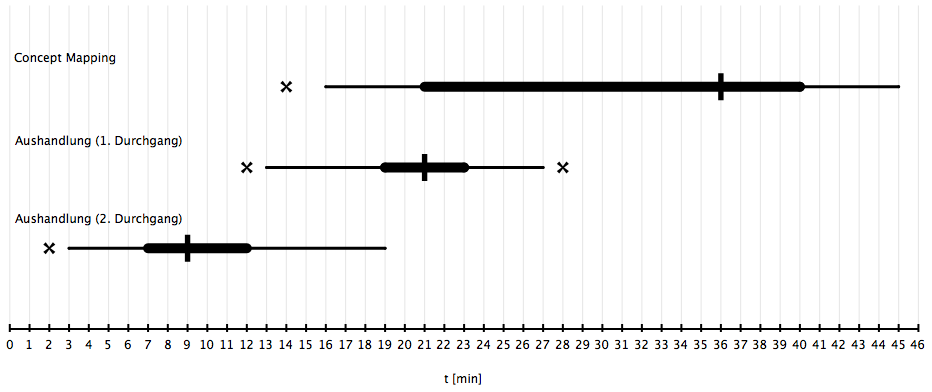
\includegraphics[width=15cm]{img/Evaluierung/usageTimeOverview.png}
	\caption{Dauer der Werkzeugverwendung -- Überblick}
	\label{fig:img_Evaluierung_usageTimeOverview}
\end{figure}

Die erhobene Dauer der Werkzeug-Verwendung teilt sich ein einen Anteil, an dem tatsächlich mit dem Werkzeug interagiert wird und einen Anteil, der anderen Tätigkeiten (wie inhaltlicher Diskussion, Bedeutungsaushandlung, \ldots) gewidmet ist. Diese beiden Anteile sind in den Evaluierungsblöcken 2 und 3 wie in den Abbildungen \ref{fig:img_Evaluierung_usageTimeConceptMapping} und \ref{fig:img_Evaluierung_usageTimeNegotiation} dargestellt verteilt. Diese beiden Evaluierungblöcke wurden prototypisch als Repräsentanten unterschiedlicher Aufgabentypen („ablauforientierte Strukturen“ in Evaluierungblock 2 und „konzeptuelle Strukturen“ in Evaluierungsblock 3) ausgewählt, die auch in den übrigen Evaluierungsblöcken zu identifizieren sind (in Evaluierungsblock 4 traten beide Typen auf, Evaluierungblock 5 erfordert die Abbildung konzeptueller Strukturen).

\begin{figure}[htbp]
	\centering
		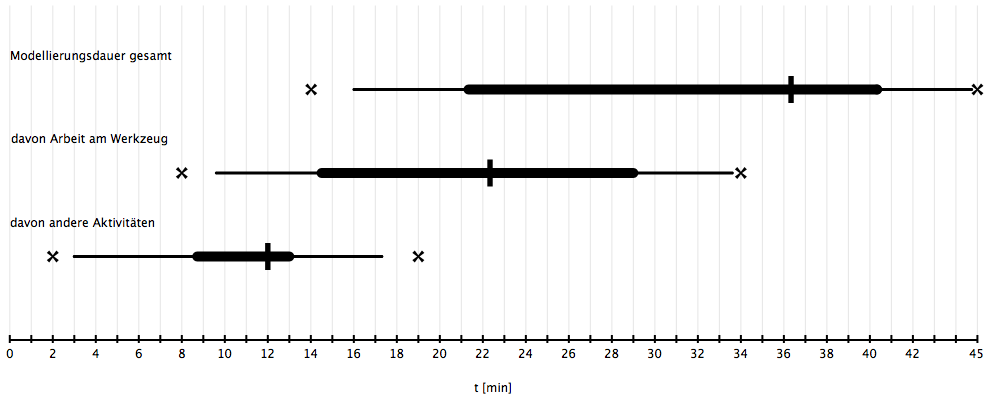
\includegraphics[width=15cm]{img/Evaluierung/usageTimeConceptMapping.png}
	\caption{Dauer der Werkzeugverwendung -- Concept Mapping}
	\label{fig:img_Evaluierung_usageTimeConceptMapping}
\end{figure}

\begin{figure}[htbp]
	\centering
		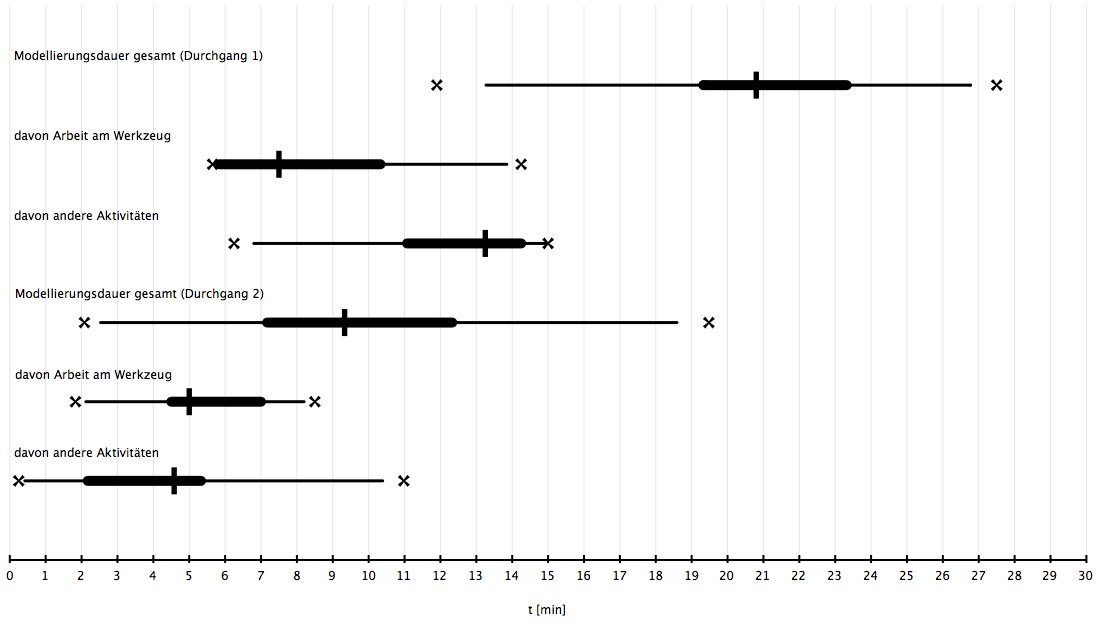
\includegraphics[width=15cm]{img/Evaluierung/usageTimeNegotiation.png}
	\caption{Dauer der Werkzeugverwendung -- Aushandlung}
	\label{fig:img_Evaluierung_usageTimeNegotiation}
\end{figure}

% subsection durchführung (end)
% section untersuchungsdesign (end)

\section{Ergebnisse} % (fold)
\label{sec:ergebnisse}

In diesem Abschnitt werden die Ergebnisse der Untersuchung gegliedert nach den oben formulierten Hypothesen dargestellt. Zu jeder Hypothese wird die Auswertung der empirischen Daten dargestellt, die Bedeutung der empirischen Belege für die Prüfung der jeweiligen Hypothese diskutiert und letztendlich das Ergebnis zusammenfassend dargestellt.  

\subsection{Repräsentation diagrammatischer Modelle} % (fold)
\label{sub:repräsentation_diagrammatischer_modelle}

Gegenstand der hier beschriebenen Untersuchung ist Hypothese \ref{hyp:diagmodelle} („Das Werkzeug ermöglicht die Repräsentation diagrammatische Modelle.“). Als Grundlage dieser Untersuchung dienen die Ergebnisse aller Evaluierungsblöcke, da die Aufgaben in allen Fällen auf die Erstellung einer Repräsentation in Form eines diagrammatischen Modells gefordert war.

Ausgewertet wird hier, ob die Ergebnisse der Modellierung jeweils als diagrammatisches Modell zu klassifizieren sind. Ein diagrammatisches Modell zeichnet nach \citep{Larkin87} aus, dass in ihm Konzepte und deren Zusammenhänge visuell-graphisch dargestellt werden. Eine Darstellung von Beziehungen kann durch die explizite Darstellung von Verbindungen zwischen Konzepten oder durch andere graphische Mittel wie Gruppierung von Konzepten in räumlicher Nähe erfolgen. Um eine eindeutige Auswertbarkeit gewährleisten zu können, wird hier auf die explizite Darstellung von Verbindungen eingeschränkt. 

\subsubsection{Auswertung} % (fold)

In allen vorliegenden Modellen wurden Konzepte als Grundelemente des diagrammatischen Modells verwendet. Das Kriterium zur Klassifizierung als diagrammatisches Modell ist im Folgenden also das Vorhandensein von Verbindungen. Bei der Auswertung ergab sich die in Tabelle \ref{tab:modelle_mit_verbindern} dargestellte Verteilung.

\begin{table}[htbp]
	\centering
	\caption{Anzahl der Modelle mit Verbindern}

\begin{tabular}{| c || c | c |}
  \hline
   Block & Modelle gesamt & Modelle mit Verbindern \\ \hline
   1 & 9 & 0 \\ 
   2 & 18 & 9 \\ 
   3 & 18 & 17 \\ 
   4 & 10 & 10 \\ 
   5 & 11 & 11 \\ \hline
   Gesamt & 66 & 47 \\ \hline
\end{tabular}
	\label{tab:modelle_mit_verbindern}
\end{table}

Insgesamt sind in 66 Modellen, die als Ergebnis vorliegen, 47 Modelle zu identifizieren, in denen explizit Verbindungen zur Darstellung von Beziehungen zwischen Konzepten verwendet werden ($71,2\%$). Eine implizite Darstellung von Beziehungen ist jedoch in allen vorliegenden Modellen zu erkennen. Nicht explizit durch Verbindungen abgebildete Beziehungen werden in allen Fällen durch die räumliche Konfiguration der Konzepte zueinander dargestellt.

\subsubsection{Diskussion} % (fold)

Legt man das Kriterium des Vorhandenseins von Verbindungen zwischen Konzepten an, so sind $71,2\%$ der betrachteten Modelle als diagrammatische Modelle zu klassifizieren. Dies erscheint vordergründig eine geringe Zahl zu sein, die gegen die allgemeine Gültigkeit der Hypothese sprechen würde. Allerdings sind in allen Modelle implizite Verbindungen zwischen Konzepten eindeutig zu identifizieren. Außerdem ist zu erkennen, dass der Anteil an diagramatischen Modellen über die Evaluierungsblöcke (und damit die Weiterentwicklung des Werkzeugs über die Zeit) hinweg stetig ansteigt, bis er in den letzten beiden Blöcken jeweils $100\%$ erreicht. Dies ist durch technische Fehlfunktionen zu erklären, die es in ersten Evaluierungsblöcken schwer bzw. teilweise unmöglich machten, explizite Verbindungen intentional zu erstellen. Unter Anbetracht dieser Erkenntnisse erscheint die Annahme der Hypothese \ref{hyp:diagmodelle} als gerechtfertigt.

Die Abbildung von Verbindungen durch räumliche Konfiguration ist Gegenstand der Prüfung von Hypothese \ref{hyp:keine_verbinder} in Kapitel \ref{cha:eval_modell} und wird dort einer näheren Betrachtung unterzogen.

\subsubsection{Ergebnis} % (fold)

\textbf{Hypothese \ref{hyp:diagmodelle} kann auf Basis der Untersuchung bestätigt werden.} Die Abbildung von Konzepten und Beziehungen zwischen diesen wurde in allen vorliegenden Modellen erfolgreich umgesetzt, wenngleich die Modellierung von expliziten Verbindungen in den ersten beiden Evaluierungsblöcken aufgrund von technischen Unzulänglichkeiten nicht durchgeführt wurde.

% subsection repräsentation_diagrammatischer_modelle (end)

\subsection{Kooperatives Arbeiten} % (fold)
\label{sub:kollaboratives_arbeiten}

Gegenstand der hier beschriebenen Untersuchung ist Hypothese \ref{hyp:kollaborativ} („Das Werkzeug ermöglicht kooperatives Arbeiten an einer Aufgabe.“). Zur Untersuchung der quantitativ beurteilbaren Aspekte wurden die Werkzeuganwendungen aus den Evaluierungsblöcken 2 ($n=18$), 3 ($n=18$) und 5 ($n=11$) herangezogen, wobei in Block 2 und 5 in Gruppen zu zwei Personen modelliert wurde (in insgesamt drei Fällen drei Personen), in Block 3 in Gruppen zu drei Personen (in drei Fällen nur zwei Personen). Zusätzlich wurden zur qualitative Beurteilung Daten aus den Blöcken 4 und 5 verwendet.

In den Evaluierungsblöcken 4 und 5 wurde hinsichtlich der subjektiven Wahrnehmung der Kooperation eine Befragung der Teilnehmer mittels eines Fragebogens durchgeführt (diese umfasste auch weitere Aspekte, die in späteren Abschnitten besprochen werden). Die Fragestellungen zur Kooperation wurde in geschlossenen Items codiert, die auf einer 7-teiligen Likert-Skala zu beantworten waren \{zu den konkreten Fragebogen-Items siehe Anhang \ref{cha:daten_der_empirischen_untersuchung}. Zusätzlich wurden offene Fragen hinsichtlich der Nützlichkeit der Werkzeugs eingesetzt, die an dieser Stelle ebenfalls hinsichtlich Aussagen zur Kooperation zwischen den Teilnehmern ausgewertet werden. 

Zur Auswertung dieser Hypothese wurden außerdem die Interaktionsanalyse berücksichtigt, die in den Evaluierungsblöcken 2 bis 5 durchgeführt wurden. Herangezogen wurden dabei jene Szenen, in denen die Kooperation zwischen den jeweiligen Teilnehmern im Vordergrund stand.

\subsubsection{Auswertung} % (fold)

Grundlage des ersten Teils der Auswertung ist die Verteilung der Modellierungsdauer zwischen den Teilnehmern. Um die unterschiedliche Gesamt-Modellierungsdauer in den einzelnen Anwendungen zu kompensieren, wurden die Berechnungen auf Basis der prozentuellen Zeitanteile der einzelnen Teilnehmer durchgeführt. Die einzelnen Datensätze wurden so sortiert, dass die anteilsmäßige Modellierungsdauer von Teilnehmer A bis Teilnehmer C (bzw. B) abnimmt. In den einzelnen Evaluierungsblöcken ergeben sich die in Abbildung \ref{fig:img_Evaluierung_timeDist} dargestellten Verteilungen.

\begin{figure}[htbp]
	\centering
		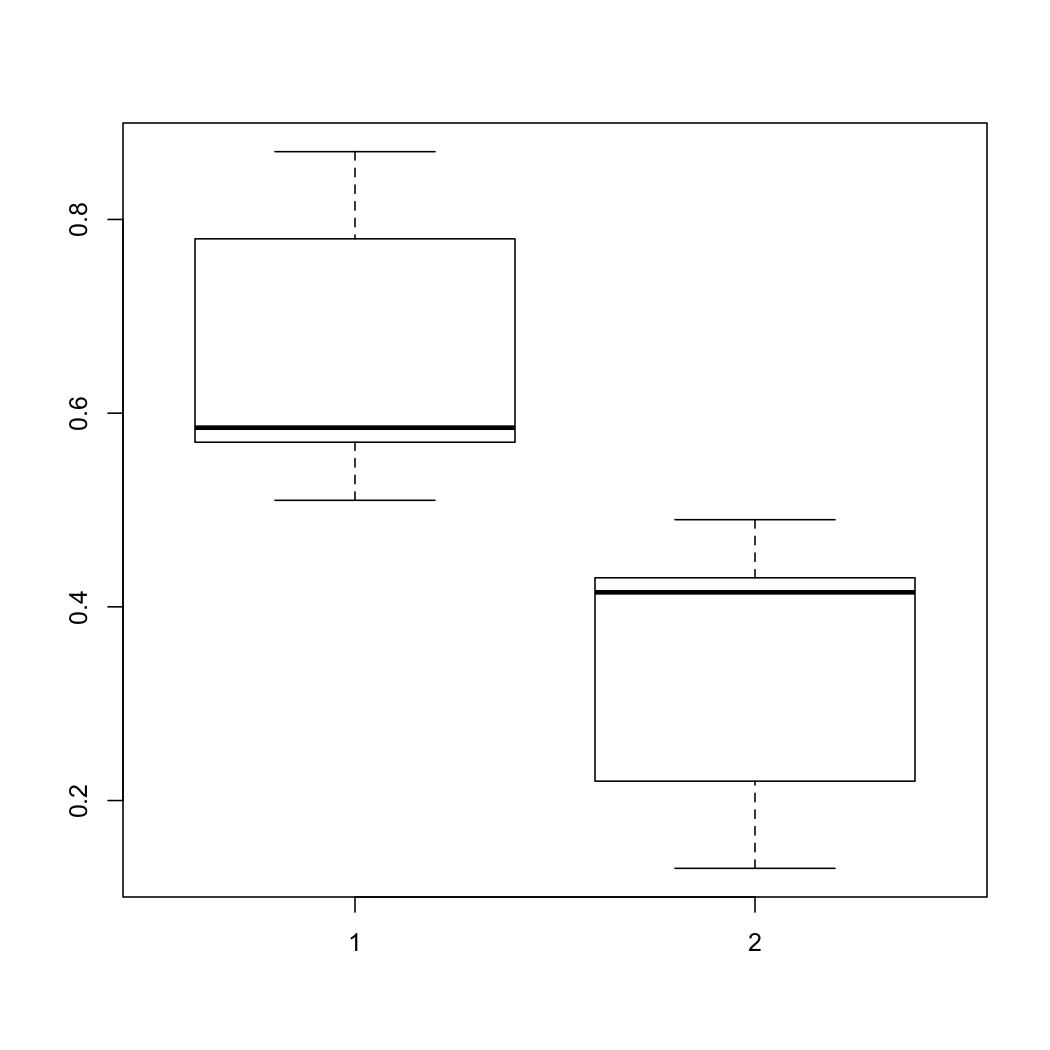
\includegraphics[height=2.5in]{img/Evaluierung/timeDist2TN.png}
		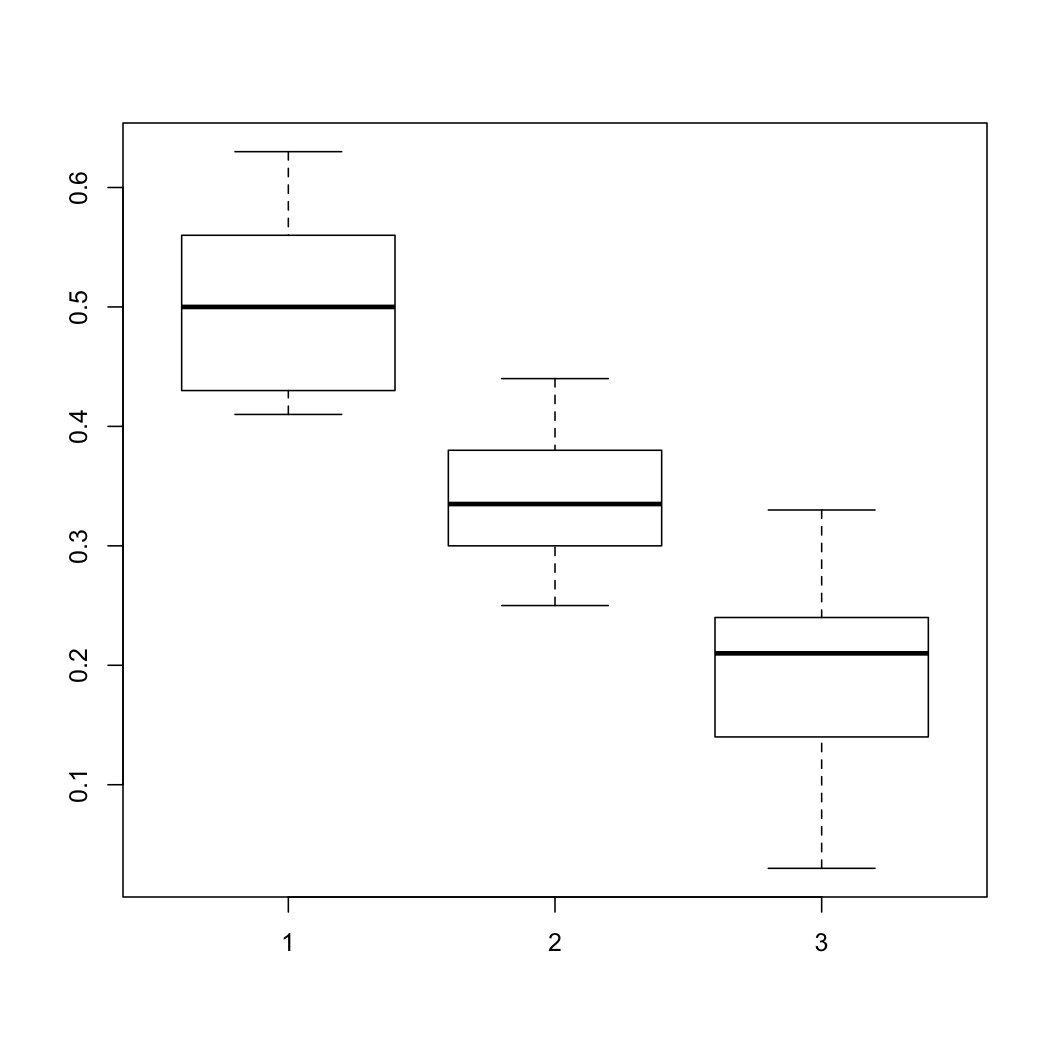
\includegraphics[height=2.5in]{img/Evaluierung/timeDist3TN.png}
	\caption[Zeitverteilung zwischen den Teilnehmern]{Zeitverteilung zwischen den Teilnehmern (1 .. TN A, 2 .. TN B, 3 .. TN C)}
	\label{fig:img_Evaluierung_timeDist}
\end{figure}

Zu prüfen ist hier, ob die Zeit-Anteile der einzelnen Teilnehmer signifikant unterschiedlich sind. Dazu wird für über dei Evaluierungsblöcke hinweg die Signifikanz zwischen den Verteilung der einzelnen Teilnehmerklassen berechnet (eine Teilnehmerklasse setzt sich aus all jenen Teilnehmern zusammen, die am längsten, am zweitlängsten bzw. am drittlängsten aktiv waren).

Für jene Anwendungen, an denen 2 Teilnehmer beteiligt waren ($n=28$) lag der durchschnittliche Zeitanteil an der Modellierung für Teilnehmer A bei $65.4\%$ ($SD=12.2\%$), jener von Teilnehmer B lag bei $34.6\%$ ($SD=12.2\%$). Die Zeitanteile unterscheiden sich damit signifikant voneinander, es ist keine Gleichverteilung der Modellierungszeiten gegeben (zweiseitiger Wilcoxon-Test für gepaarte Stichproben: $V=351, p<0.005$\footnote{Der t-Test kann nicht angewandt werden, da beide Stichproben nicht normalverteilt sind (Shaprio-Wilk-Test: $W_{TN A}=0.826, p_{TN A}<0.005$, $W_{TN B}=0.820, p_{TN B}<0.005$).}.

Für jene Anwendungen, an denen 3 Teilnehmer beteiligt waren ($n=19$) lag der durchschnittliche Zeitanteil an der Modellierung für Teilnehmer A bei $49.3\%$ ($SD=7.2\%$), jener von Teilnehmer B lag bei $33.1\%$ ($SD=5.9\%$) und jener von Teilnehmer C lag bei $17.6\%$ ($SD=8.2\%$) . Die Zeitanteile unterscheiden sich damit signifikant voneinander, es ist keine Gleichverteilung der Modellierungszeiten gegeben (Kruskal-Wallis-Test für mehr als zwei Stichproben: $\chi^{2}=43.65, df=2, p<0.005$\footnote{Der t-Test könnte grundsätzlich für die paarweise Testung ebenfalls angewandt werden, da für alle drei Stichproben nicht davon ausgegangen werden kann, dass sie nicht normalverteilt sind (Shaprio-Wilk-Test: $W_{TN A}=0.9075, p_{TN A}=0.078$, $W_{TN B}=0.9523, p_{TN B}=0.463$, $W_{TN C}=0.9523, p_{TN C}=0.463$) und auch der Test der Varianzen eine Gleichheit derselben vermuten lässt (paarweiser F-Test: $F_{AB}=1.47, p_{AB}=0.434$, $F_{AC}=0.778, p_{AC}=0.610$, $F_{BC}=0.528, p_{BC}=0.199$). Die errechneten paarweisen Werte für t weisen ebenfalls jeweils einen signifikanten Unterschied der Zeitanteile hin ($t_{AB}=7.32, t_{AC}=12.30, t_{BC}=6.49$, $p$ jeweils $<0.005$)}).
6666*2
Zudem konnten in der Videoanalyse der Evaluierungsblöcke 2, 3, 4 und 5 vielfach Situationen identifiziert werden, in denen das Modell auf der Tischoberfläche von den Teilnehmern als Referenz für den Austausch über die abgebildeten Inhalte herangezogen wurden oder in denen mehrere Teilnehmer gleichzeitig das Modell manipulierten. In der Folge werden prototypisch einige Situationen dargestellt, die derartige Interaktionsabläufe zeigen\footnote{Die ausgewählten Transkripte stammen aus Evaluierungsblock 3. Sämtliche Transkripte sind unter den in Anhang \ref{cha:daten_der_empirischen_untersuchung} angeführten Quellen zu beziehen.}:

\paragraph{Beispiel für gleichzeitige Manipulation} % (fold)
\begin{transkript}
	\textbf{A:} Sollen wir die beiden auch verbinden? \\
	\textbf{C:} Sicher. \emph{\textbf{(greift zu rotem Block)}} \\
	\textbf{A:} OK. \emph{\textbf{(greift zu blauem Block)}} \\
	\emph{\textbf{A und C schieben die Blöcke zusammen und anschließend wieder in die ursprüngliche Position. Anschließend setzt B den nächsten blauen Block auf die Arbeitsfläche, und verbindet ihn mit dem roten Block.}} \\
\end{transkript}

\paragraph{Beispiel für Referenzierung des Modells} % (fold)
\begin{transkript}
	\textbf{B:} Die Übung \emph{\textbf{(deutet auf roten Block)}} ist eigentlich nicht notwendig. \\
	\textbf{A:} Naja es ist halt unter einem schönen Knoten. \\
	\textbf{C:} Nennen wir das \emph{\textbf{(tippt auf roten Block)}} Ziele. \\
	\textbf{A:} Nein wieso? Ich kann ja mehrere Bedeutungen für das \emph{\textbf{(deutet auf roten Block)}} verwenden. Das ist doch egal. Das sagt ja nichts aus. \\
	\textbf{C:} Aber wir können das \emph{\textbf{(deutet auf roten Block)}} weggeben und sagen das sind die Ziele. Was ist das Ziel. \\
	\textbf{A:} Das können wir machen, oder wir legen einfach einen roten dazu \emph{\textbf{(deutet an wo der rote Block liegen würde)}} und schreiben es hin. \\
	\emph{A verschiebt den roten Block um Platz für einen neuen Block zu schaffen.} \\
\end{transkript}

\paragraph{Beispiel für gleichzeitige Manipulation} % (fold)
\begin{transkript}
	\emph{Die Teilnehmer haben zuvor alle Blöcke beschriftet und wollen sie nun verbinden bzw. in die richtige Position bringen.} \\
	\textbf{B:} So und jetzt müssen wir eigentlich \ldots \emph{(greift zum ersten Block und schiebt ihn zum Knotenpunkt, um ihn zu verbinden, danach bringt er den Block wieder in seine ursprüngliche Position)} \\
	\textbf{C:} Jawohl. \\
	\emph{\textbf{Teilnehmer B wiederholt Vorgang mit dem zweiten Block. Teilnehmer C greift inzwischen zum dritten Block um es B nachzumachen. B nimmt anschließend den nächsten Block und verbindet ihn. Den letzten Block verbindet wieder C.} Beim zurückschieben verschwindet die Verbindung von der Arbeitsfläche.} \\
	\textbf{A:} Das erkennt er nicht. \emph{(schiebt den Block wieder ein Stück zurück)} \\
	\emph{System zeigt Verbindung wieder an.} \\
	\textbf{C:} Passt. \emph{Schiebt Block wieder zurück.} \\
	\textbf{A:} So und jetzt noch schön anordnen. \\
	\emph{\textbf{A greift die unteren Blöcke und richtet sie in einer Linie aus, während C den ober Block zentriert.} System reagiert etwas verzögert. B lacht.} \\
	\textbf{A:} Ok. Passt. \\
	\emph{In der Folge beraten die Teilnehmer über die weitere Vorgangsweise.} \\
\end{transkript}

\paragraph{Beispiel für Referenzierung des Modells} % (fold)
\begin{transkript}
	\emph{Teilnehmer diskutieren über die beiden Modellierungssprachen.} \\
	\textbf{A:} In der Softwareentwicklung würde man das Analyse \emph{\textbf{(deutet auf oberen Teil der Arbeitsfläche)}} und das Design \emph{\textbf{(deutet auf unteren Teil der Arbeitsfläche)}} nennen. \\
	\textbf{B:} Genau. \\
	\textbf{A:} Und dann hinterlegst du es mit deinen mathematischen Modellen \emph{\textbf{(deutet Modelle mit Handbewegung an)}} in der Implementierung und dann kann ich es ausführen. \\
	\textbf{B:} Ja. Alles ablauforientiert das Ganze. \\
	\textbf{A:} \emph{\textbf{(deutet auf blauen Baustein)}} Genau, von der Sicht her. Die Sicht die es einnimmt \emph{\textbf{(deutet auf gelbe Blöcke}}) ist genau dasselbe aber der Scope vom Zeitpunkt ist genau. \\
	\textbf{B:} unterschiedlich \\
	\textbf{A:} Genau SeeMe, Aris \emph{\textbf{(deutet Modelle an)}} und dann Workflow Systeme im Wesentlichen. \\
\end{transkript}

\subsubsection{Diskussion} % (fold)

In der Verteilung der Zeitanteile der Beteiligung an der Modellierung zeigt sich, dass der Anteil von Teilnehmer A (dem Teilnehmer mit dem jeweils höchsten Zeitanteil) signifikant höher ist als jener von Teilnehmer B. In jenen Fällen, in denen drei Teilnehmer beteiligt sind, ist der Zeitanteil des am kürzesten beteiligten Teilnehmers signifikant geringer als jener der anderen beiden. Dieses Ergebnis scheint darauf hinzudeuten, dass für Anwendungssituationen mit mehreren Teilnehmern eine Beteiligung im gleichen Ausmaß nicht erwartet werden kann. Insgesamt spricht dieses Ergebnis also eher gegen für die Bestätigung der Hypothese. 

Das Ergebnis ist aber insofern zu relativieren, als das statistisch signifikante Gleichverteilung nicht erwartet werden kann. Betrachtet man die Mittelwerte der Zeitanteile der Teilnehmer, so zeigt sich, dass -- zumindest für Anwendungen mit zwei Teilnehmern -- eine Beteiligung jeweils durch alle Teilnehmer gegeben ist. Der höhere Zeitanteil von Teilnehmer A ist unter Umständen auch auf den exklusiven Zugriff auf die zur Benennung von Modellierungsblöcken notwendige Tastatur zu erklären. Die Bedienung der Tastatur wurde nur in wenigen Fällen geteilt, so dass ein Teilnehmer durch die Durchführung der Benennungstätigkeit naturgemäß einen stärkeren Anteil an der Arbeitszeit in Anspruch nimmt. Bei drei Teilnehmern zeigt sich jedoch eine deutliche Abnahme des Zeitanteils für jenen Teilnehmer, der den geringsten Zeitanteil in Anspruch nahm. Dieser Effekt verstärkt sich -- wie aus den Beobachtungen der Anwendungen im Evaluierungsblock 4 zu erkennen -- für Anwendungen mit mehr als drei Teilnehmern. Hier sind tendentiell zwei Beteiligte zu identifizieren, die zusammen mehr als zwei Drittel der Modellierungszeit für sich in Anspruch nehmen.  

In der Befragung der Benutzer hinsichtlich der wahrgenommenen Möglichkeit zur Kooperation wird deutlich, dass diese durchwegs als hoch eingeschätzt wird (dies gilt sowohl für die Anwendungen mit zwei Teilnehmern in Block 5 als auch für die Anwendungen mit drei und mehr Teilnehmern in Block 4). Auch in den qualitativen Rückmeldungen zur Kooperation wird das Werkzeug hinsichlich seiner Wirkung positiv beurteilt. Auch die Antworten auf die offenen Fragestellungen zeigen eine vorwiegend positive Einschätzung der Wirkung des Werkzeugs auf die Kooperation zwischen den Teilnehmern. Das Ergebnis der Befragung spricht also insgesamt für die Bestätigung der Hypothese.

Auch die Ergebnisse der Videoanalyse deuten auf eine kooperationsunterstützende Wirkung des Werkzeugs hin. Zu nennen ist hierbei vor allem die vielfache Verwendung der Modellelemente als physischer Ankerpunkt, an dem Diskussionbeiträge durch Zeigen oder Deuten festgemacht werden und so den anderen Teilnehmern der Bezugsgegenstand verdeutlicht wird. Dieses Verhalten bei der Modellbildung war in der vergleichenden Anwendung der rein rechnerbasierten CMapTools in Evaluierungsblock 5 in weitaus geringerem Ausmaß zu beobachten. Auch die simultane Manipulation am Modell durch mehrere Teilnehmer trat wiederholt auf. Dabei handelte es sich selten um vollständig voneinander entkoppelte Aktivitäten, in den meisten Fällen wurde simultan jener Modellteil manipuliert, der aktuell Gegenstand der Diskussion war. Durch die bei rein rechner-gestützten Modellierungswerkzeugen exklusiven Interaktionsmöglichkeit durch die Maus ist dieses Verhalten dort nicht zu beobachten und deutet auf einen auf das Werkzeug zurückzuführenden Effekt hin.   

Insgesamt kann die hier untersuchte Hypothese auf Basis der durchgeführten Untersuchungen deshalb bestätigt werden.

\subsubsection{Ergebnis} % (fold)

\textbf{Hypothese \ref{hyp:kollaborativ} kann auf Basis der Untersuchung bestätigt werden.} Der Zeitanteil an der Modellbildung ist für Anwendungen mit zwei Teilnehmern weitgehend gleichverteilt. Bei mehr als zwei Anwendern ist die Gleichverteilung nicht mehr gegeben, die Teilnehmer haben dennoch durchwegs (unabhängig von der Anzahl der Teilnehmer bei einer Anwendung) den Eindruck sich einbringen zu können und gut zusammenarbeiten zu können.

% subsection kollaboratives_arbeiten (end)

\subsection{Einsetzbarkeit in unterschiedlichen Kontexten} % (fold)
\label{sub:einsetzbarkeit_in_unterschiedlichen_kontexten}

Gegenstand der hier beschriebenen Untersuchung Hypothese \ref{hyp:kontexte} („Das Werkzeug ist gleichwertig für Modellierungsaufgaben in unterschiedlichen Kontexten einsetzbar.“). Als Grundlage dieser Untersuchung dienen die Ergebnisse der Evaluierungsblöcke 2, 3, 4 und 5. Die Anwendungskontexte unterscheiden sich weitgehend zwischen den Blöcken. In Block 2 werden Ablaufplanungen im universitären Lern-Kontext behandelt, die Blöcke 3 und 5 bilden Aufgaben zur Reflexion von Lerninhalten ab. Block 4 zeigt den Einsatz des Werkzeugs im organisationalen Kontext, wobei hier sowohl die Aufbau- als auch die Ablauforganisation (zumeist nicht trennbar) behandelt wurden. Zur Auswertung werden also drei Kontexte (Block 2, Blöcke 3 und 5 sowie Block 4) betrachtet. In den Blöcken 4 und 5 wurden die Teilnehmer zusätzlich hinsichtlich der Zufriedenheit mit der Abbildung ihrer mentalen Modelle befragt. Auch diese Ergebnisse dienen der Prüfung dieser Hypothese.

\subsubsection{Auswertung} 

Im quantitativen Teil der hier durchgeführten Auswertung wurde die Korrelation zwischen der Modellierungszeit und der Modellgröße in den unterschiedlichen Evaluierungsblöcken berechnet. Abbildung \ref{fig:img_Evaluierung_correlation} zeigt den Zusammenhang graphisch.

\begin{figure}[htbp]
	\centering
		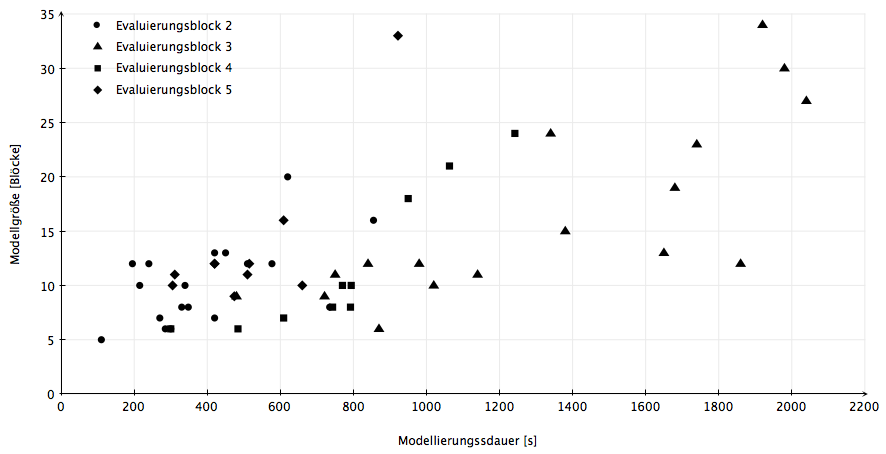
\includegraphics[width=15cm]{img/Evaluierung/correlation.png}
	\caption{Zusammenhang zwischen Modellgröße und Modellierungsdauer}
	\label{fig:img_Evaluierung_correlation}
\end{figure}

Über alle Evaluierungsblöcke hinweg ($n=57$) ergibt sich mit einem Korrelationskoeffizient nach Spearman\footnote{Der Korrelationskoeffizient nach Pearson kann nicht angewandt werden, da beide Stichproben nicht normalverteilt sind (Shapiro-Wilk-Test: $W_{Zeit}=0.880, p_{Zeit}<0.005$, $W_{Größe}=0.829, p_{Größe}<0.005$)} von $0.60019$ ein signifikant positiver Zusammenhang zwischen den beiden Messgrößen (Test auf positive Korrelation: $S=11082.87, p<0.005$).

Bei der Befragung der Benutzer in den Blöcken 4 ($n=13$) und 5 ($n=24$) wurde unter anderem deren Zufriedenheit mit dem Modellierungsergebnis sowie der Anwendung der Werkzeugs zur Lösung der Aufgabenstellung qualitativ erhoben. In Evaluierungsblock 4 gaben 11 Teilnehmer an, mit dem Modellierungsergebnis zufrieden gewesen zu sein. Ein Teilnehmer war unzufrieden, einer beantwortete die Frage nicht. Insgesamt wurden von 9 Teilnehmern Begründungen angegeben, die im Folgenden inhaltlich gruppiert dargestellt sind:

\begin{itemize}
	\item pos: kooperatives Arbeiten möglich (3x)
	\item pos: neue Erkenntnisse gewonnen (2x)
	\item pos: Ergebnis entspricht den Vorstellungen (2x)
	\item neg: zu große Teile, zu kleine Oberfläche (2x)
\end{itemize}

11 Teilnehmer gaben an, mit dem Modellierungsverlauf zufrieden gewesen zu sein, ein Teilnehmer war nicht zufrieden, ein Teilnehmer beantwortete die Frage nicht. Insgesamt wurden von 8 Teilnehmern Begründungen angegeben, die im Folgenden inhaltlich gruppiert dargestellt sind:

\begin{itemize}
	\item pos: kooperatives Arbeiten möglich (3x)
	\item pos: Kommunikation gefördert, gemeinsame Sichtweise entwickelt (2x)
	\item pos: Experimentieren ist möglich (1x)
	\item pos: spielerisches Modellieren möglich (1x)
	\item neg: zu große Teile, zu kleine Oberfläche (1x)
	\item neg: Werkzeug ist umständlich (1x)
	\item neg: Werkzeug technisch instabil (1x)
\end{itemize}

In Evaluierungsblock 5 gaben 18 Teilnehmer an, mit dem Modellierungsergebnis zufrieden gewesen zu sein. 6 Teilnehmer waren unzufrieden. 23 Teilnehmer begründeten ihre Entscheidung. Die Begründungen sind im Folgenden inhaltlich gruppiert dargestellt:

\begin{itemize}
	\item pos: Modell war vollständig (5x)
	\item pos: Aufgabe gut gelöst (5x)
	\item pos: Modell war verständlich (2x)
	\item pos: Ergebnis entspricht den Vorstellungen (2x)
	\item pos: rasch Modellierung war möglich (1x)
	\item neg: Werkzeug technisch instabil (4x)
	\item neg: Modell war zu ungenau (3x)
	\item neg: Modell war unübersichtlich (2x)
\end{itemize}

20 Teilnehmer gaben an, mit dem Modellierungsverlauf zufrieden gewesen zu sein, 4 Teilnehmer waren nicht zufrieden. Alle 24 Teilnehmer begründeten ihre Entscheidung. Die Begründungen sind im Folgenden inhaltlich gruppiert dargestellt:

\begin{itemize}
	\item pos: kooperatives Arbeiten möglich (11x)
	\item pos: Kommunikation gefördert (7x)
	\item pos: Werkzeug einfach zu bedienen (5x)
	\item pos: Verwendung unterhaltsam (3x)
	\item pos: zügiges Arbeiten möglich (3x)
	\item pos: gute Aufgabenteilung (1x)
	\item neg: Werkzeug technisch instabil (3x)
	\item neg: Werkzeug ist umständlich (1x)
	\item neg: unstrukturiertes Vorgehen (1x)
\end{itemize}

\subsubsection{Diskussion} 

Der Korrelationskoeffizient zwischen Modellgröße und Modellierungsdauer deutet bei einer Berechnung über alle Evaluierungsblöcke hinweg mit einem Wert von $0.696$ auf eine signifikant positive Korrelation zwischen diesen beiden Parametern hin (einseitiger Test auf signifikant positive Korrelation der Merkmale: $S=11082.87, p<0.005$). Da damit unabhängig von der Modellierungsaufgabe offensichtlich ein Zusammenhang besteht, stützt dies die Hypothese, das sich das Werkzeug für den Einsatz in unterschiedlichen Kontexten eignet. Auch die in Abschnitt \ref{sub:gewöhnung_an_das_werkzeug} verwendeten „normierten“ Modellierungszeiten (Modellierungdauer im Verhältnis zur Modellgröße, also im Wesentlichen Zeitaufwand pro Block) zeigen für die dort gegenübergestellten Blöcke 2 und 3 keinen signifikanten Unterschied im Aufwand bei der Modellierung, obwohl die Anwendungen aus unterschiedlichen Kontexten stammen.

Bei der qualitativen Betrachtung der Rückmeldungen der Benutzer hinsichtlich der Zufriedenheit mit dem Modellierungsverlauf und Ergebnis zeigen sich unabhängig von jeweiligen Anwendungskontext überwiegend positiv zu wertende Rückmeldungen. Betrachtet man die mehrfach genannten Begründungen der Einschätzungen, gleichen sich sowohl die positiven als auch die negativen Rückmeldungen in den beiden Anwendungskontexten. Dies spricht für die Bestätigung der untersuchten Hypothese.

Zusammenfassend kann Hypothese \ref{hyp:kontexte} also auf Basis der Ergebnisse der durchgeführten Untersuchungen bestätigt werden.

\subsubsection{Ergebnis} 

\textbf{Hypothese \ref{hyp:kontexte} kann auf Basis der Untersuchung bestätigt werden.} Die quantitative Untersuchung der Korrelation zwischen Modellgröße und Modellierungsdauer zeigt unabhängig vom Anwendungskontext eine signifikant positive, relativ stark ausgeprägte Korrelation, was darauf hinweist, das der Aufwand zur Modellerstellung unabhängig von Aufgabenstellung und Anwendungskontext relativ stabil bleibt. Auch die qualitativen Rückmeldungen der Teilnehmer aus unterschiedlichen Anwendungskontexten gleichen sich im Wesentlichen, so dass das Werkzeug unabhängig vom Anwendungskontext immer ähnliche positive bzw. negative Effekte zu haben scheint.

% subsection einsetzbarkeit_in_unterschiedlichen_kontexten (end)

\subsection{Wiederherstellung vergangener Modellzustände} % (fold)
\label{sub:wiederherstellung_vergangener_modellzustände}

Gegenstand der hier beschriebenen Untersuchung ist Hypothese \ref{hyp:wiederherstellung} („Die Möglichkeit der Wiederherstellung vergangener Modellzustände fördert die Bereitschaft alternative Repräsentationen auszuprobieren.“). Als Grundlage dieser Untersuchung dienen die Ergebnisse der Evaluierungsblöcke 2 bis 5, da die Funktion zur Wiederherstellung vergangener Modellzustände erst in diesen Blöcken funktionsfähig zur Verfügung stand.

\subsubsection{Auswertung} 

Für alle Anwendungen des Werkzeugs in den Evaluierungsblöcken 2 bis 5 wurde hier untersucht, wie oft die Möglichkeit zur Wiederherstellung vergangener Modellzustände eingesetzt wurde, um alternative Modellierungswege auszuprobieren. Nicht berücksichtigt wurden Einsätze derselben Funktion, die zur Korrektur von Modellierungsfehlern durch Fehlerkennungen des Systems verwenden wurden (verstärkt in den Evaluierungsblöcken 2 und 3 aufgetreten, in 4 und 5 durch Stabilisierung der Erkennungsleistung nicht mehr relevant). Die Verteilung des Einsatzes der Funkion ist in absoluten Zahlen in Tabelle \ref{tab:anzahl_wiederherstellung} für jeden Evaluierungsblock angeführt

\begin{table}[htbp]
	\centering
	\caption{Anzahl des Einsatzes der Wiederherstellungsfunkion}
\begin{tabular}{| c || c | c | c | c |}
  \hline
   EB    & 0 E. & 1 E. & 2 E. & 3+ E. \\ \hline
   2     & 18 & 0 & 0 & 0 \\ 
   3     & 14 & 4 & 0 & 0 \\ 
   4     & 10 & 0 & 0 & 0 \\ 
   5     & 10 & 1 & 0 & 0 \\ \hline
   Ges.  & 52 & 5 & 0 & 0 \\ \hline
\end{tabular} \\
\footnotesize EB \ldots Evaluierungsblock, x E.\ldots x Einsätze der Wiederherstellungsfunktion
	\label{tab:anzahl_wiederherstellung}
\end{table}

Die Wiederherstellungsfunktion wurde also insgesamt in $8.77\%$ der Fälle ($n=57$) eingesetzt und kam maximal einmal je Anwendung zum Einsatz.  Aus den Videoanalysen ist außerdem erkennbar, dass die Wiederherstellungsfunktion -- falls ihre Verwendung überhaupt in Betracht gezogen wird -- in den meisten Fällen lediglich zur Fehlerkorrektur eingesetzt wird. (in 52 Anwendungen wurde die Wiederherstellungsfunkion in 37 Fällen -- $71.2\%$ -- mindestens einmal zur Korrektur von Erkennungsfehlern und 5 mal zur Korrektur von inhaltlich verworfenen Modellierungswegen verwendet).

Bei der in den Blöcken 1, 4 und 5 durchgeführten Befragung der Teilnehmer hinsichtlich der Erfahrungen mit dem Werkzeug wurde unter anderem nach als besonders nützlich empfundenen Funktionen bzw. Eigenschaften des Werkzeugs gefragt. Die Wiederherstellungsfunktion wurde in diesem Zusammenhang von keinem Teilnehmer ($n=55$) erwähnt. 

\subsubsection{Diskussion} 

Die Ergebnisse der Auswertung der Untersuchung zu dieser Hypothese zeigt ein geringes Ausmaß der Verwendung der Wiederherstellungsfunktion zum Zwecke der Erstellung von Modellalternativen. Die Funktion wurde in $71.2\%$ der Anwendungen verwendet, was für ein hohes Bewusstsein über deren Existenz spricht. Lediglich in $8.77\%$ der Anwendungen wurde die Funktion zur Verfolgung alternativer Modellierungswege eingesetzt, in $61.5\%$ der Anwendungen wurde sie lediglich zur Fehlerkorrektur verwendet. Auch in der qualitativen Erhebung der als nützlich wahrgenommenen Werkzeugfunktionalitäten wurde die Wiederherstellungsfunktion in keinem Fall genannt. Auf Basis dieser Ergebnisse kann die Hypothese nicht bestätigt werden. 

\subsubsection{Ergebnis} 

\textbf{Hypothese \ref{hyp:wiederherstellung} kann auf Basis der Untersuchung nicht bestätigt werden.} Die Wiederherstellungsfunktion wird nur in unter $10\%$ der untersuchten Anwendungen  zur Verfolgung alternativer Modellierungswege genutzt. Die Funktion wird außerdem von den Anwendern bei der Frage nach den als nützlich wahrgenommene Funktionen nicht genannt.

% subsection wiederherstellung_vergangener_modellzustände (end)

\subsection{Nicht-Behinderung} % (fold)
\label{sub:nicht_behinderung}

Gegenstand der hier beschriebenen Untersuchung ist Hypothese \ref{hyp:behinderung} („Das Werkzeug behindert die Modellbildung nicht.“). Als Grundlage dieser Untersuchung dienen die Ergebnisse der Evaluierungsblöcke 2 bis 5, da sich das Werkzeug erst in diesen Blöcken hinsichtlich der Funktionalität in vollständigem Zustand befand. Zu berücksichtigen ist bei der Auswertung, dass im Laufe der Evaluierungsblöcken 4 und 5 eine Überarbeitung der Implementierung vorgenommen wurde, mittels der das Auftreten von Fehlerkennungen verringert werden konnte und deren Korrektur weniger aufwändig wurde. Befragungen der Modellierenden hinsichtlich einer etwaigen Behinderung durch das Werkzeug wurden in den Blöcken 1, 4 und 5 durchgeführt, wobei lediglich die Anmerkungen aus den letzen beiden Blöcken für den aktuellen Entwicklungsstand des Werkzeugs relevant sind.

\subsubsection{Auswertung} 

In Tabelle \ref{tab:fehlfunktionen} wird gegliedert nach Evaluierungsblocken dargestellt, wie oft es in einer einzelnen Anwendung zu Fehlfunktionen in der Erkennung kam, die den Modellierungsfluss unterbrachen. Als Fehlerkennungen wurde das Verschwinden von Blöcken oder Fehlzuordnungen von Benennungen sowie die unbeabsichtigte oder von System eigenständig vorgenommene Erstellung oder Entfernung von Verbindern bzw. Richtungspfeilen eingeordnet. Zusätzlich wurden Systemabstürze als massive Unterbrechung, die zum Gesamtverlust des bis zum Zeitpunkt des Absturzes erstellten Modells führten, separat ausgewertet.

\begin{table}[htbp]
	\centering
	\caption{Fehlfunktionen und Abstürze des Werkzeugs}
\begin{tabular}{| c || c || c | c | c | c || c |}
  \hline
   EB    & Anw. & 0 Ff. & 1-3 Ff. & 4-6 Ff. & 7+ Ff. & Systemabstürze \\ \hline
   2     & 18 & 0 &  8 &  5 &  5 &  4 \\ 
   3     & 18 & 1 & 10 &  4 &  3 &  5 \\ 
   4     & 10 & 0 &  2 &  2 &  5 &  1 \\ 
   5     & 11 & 0 &  3 &  3 &  4 &  5 \\ \hline
   Ges.  & 57 & 1 & 23 & 14 & 17 & 15 \\ \hline
\end{tabular} \\
\footnotesize EB \ldots Evaluierungsblock, Anw. \ldots Anzahl der Anwendungen, x Ff.\ldots x Fehlfunktionen
	\label{tab:fehlfunktionen}
\end{table}

In der Gesamtheit der betrachteten Anwendungen ($n=57$) ergibt sich folgende Verteilung der Anzahl der Fehlerkennungen je Anwendung, die auch in Abbildung \ref{fig:img_Evaluierung_fehlerkennungen} graphisch dargestellt ist. In $1.75\%$ der Fälle ($n_{0}=1$) trat keine Fehlerkennung während der Anwendung auf. In $40.35\%$ der Fälle ($n_{1-3}=23$) traten zwischen 1 und 3 Fehlerkennungen auf. 4-6 Fehlerkennungen konnten in $24.56\%$ der Fälle ($n_{4-6}=14$) festgestellt werden. 7 oder mehr Fehlerkennungen traten in $29.82\%$ der Fälle ($n_{7+}=17$) auf. In $26.32\%$ der Fälle ($n_{Absturz}=15$) kam es zu Systemabstürzen, wobei diese in 10 Fällen nach Ende des eigentlichen Modellierungsvorgangs auftraten.

\begin{figure}[htbp]
	\centering
		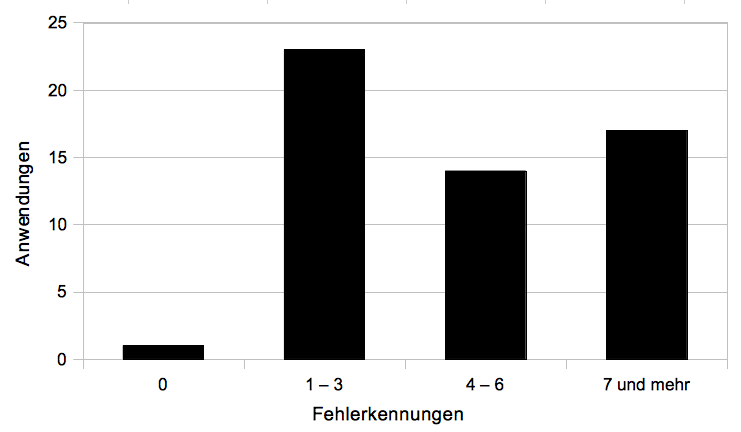
\includegraphics[width=10cm]{img/Evaluierung/fehlerkennungen.png}
	\caption{Verteilung der Anzahl der Fehlerkennungen je Anwendung -- Übersicht}
	\label{fig:img_Evaluierung_fehlerkennungen}
\end{figure}

In der Benutzerbefragung in den Evaluierungsblöcken 4 und 5 wurde in offenen und geschlossenen Fragen nach der Wirkung des Werkzeugs bei der Modellbildung befragt (Abschnitte „Nutzerfreundlichkeit“ und „Zufriedenheit des Modellierers“ in Block 4 -- siehe Anhang \ref{sub:fb_eval4} -- und Abschnitte „wahrgenommene Einfachheit der Benutzung des Werkzeugs“ und „Zufriedenheit des Modellierers“ in Block 5 -- siehe Anhang \ref{sub:fb_eval5}). Die für die Prüfung der hier betrachteten Hypothese sind folgende geschlossene Items relevant:

\begin{enumerate}
	\item Die Anwendung des Werkzeugs ist frustrierend (Skala gedreht).
	\item Die Anwendung des Werkzeugs fällt mir leicht.
	\item Die Anwendung des Werkzeugs ist anstrengend (Skala gedreht).
	\item Um mit dem Werkzeug gut zurecht zu kommen, hätte ich intensivere Vorbereitung benötigt (Skala gedreht).
	\item Die Bedienung des Werkzeugs ist intuitiv.
	\item Das Werkzeug ist einfach zu bedienen.
	\item Die benötigte Zeit um das Modell zu erstellen empfand ich als angemessen.
\end{enumerate}

Insgesamt wurden $n=37$ Teilnehmer befragt. Die Ergebnisse sind in Tabelle \ref{tab:behinderung} und Abbildung \ref{fig:img_Evaluierung_behinderung} zusammengefasst dargestellt. Neben dem Mittelwert und der Standardabweichung wurde für jedes Item auch geprüft, ob die Einschätzung als signifikant positiv zu bezeichnen ist. Dazu wurde ein einseitiger Wilcoxon-Test für die Stichprobe gegenüber dem Skalenmittelwert 4 durchgeführt\footnote{Der Wilcoxon-Test muss angewandt werden, da die Stichprobe in allen sieben Fällen nicht normalverteilt ist (Shapiro-Wilk-Test: $W_{1}=0.877, p{1}<0.005$, $W_{2}=0.798, p{2}<0.005$, $W_{3}=0.871, p{3}<0.005$, $W_{4}=0.764, p{4}<0.005$, $W_{5}=0.862, p{5}<0.005$, $W_{6}=0.833, p{6}<0.005$, $W_{7}=0.844, p{7}<0.005$)}.

\begin{table}[htbp]
	\centering
	\caption{Befragung über die Wirkung des Werkzeugs -- Itemauswertung}

\begin{tabular}{| c || c | c || c | c |}
  \hline
   Item & M & SD & $V_{M<4}$ & $p_{M<4}$ \\ \hline
   1* & $2.89$ & $1.76$ & $100$ & $<0.005$ \\ 
   2  & $2.19$ & $1.29$ & $20$ & $<0.005$ \\ 
   3* & $2.65$ & $1.49$ & $49$ & $<0.005$ \\ 
   4* & $2.08$ & $1.28$ & $33.5$ & $<0.005$ \\ 
   5  & $2.78$ & $1.49$ & $70.5$ & $<0.005$ \\ 
   6  & $2.32$ & $1.21$ & $27$ & $<0.005$ \\ 
   7  & $2.16$ & $1.35$ & $20.5$ & $<0.005$ \\ \hline
\end{tabular} \\ 
	\footnotesize * \ldots Item gedreht
	\label{tab:behinderung}
\end{table}

\begin{figure}[htbp]
	\centering
		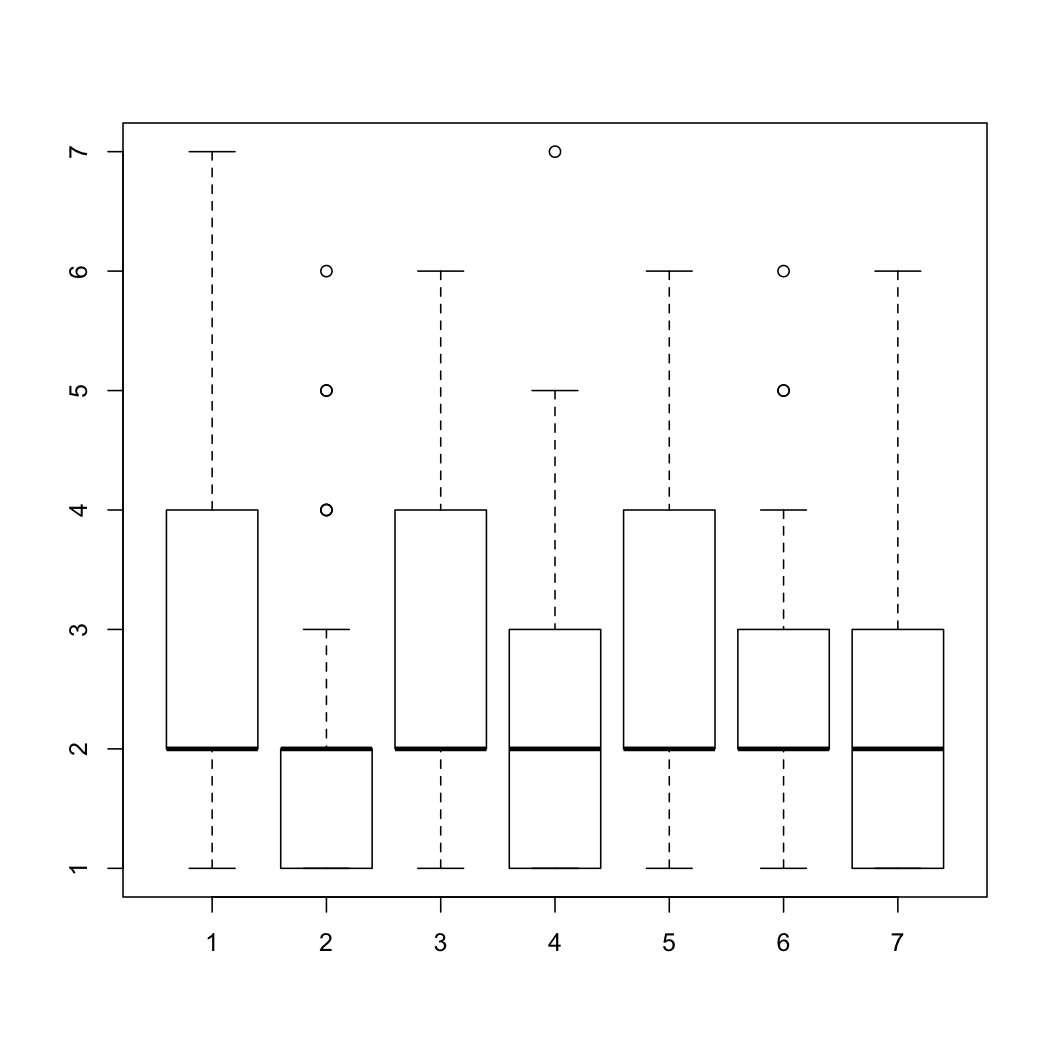
\includegraphics[height=3in]{img/Evaluierung/behinderung.png}
	\caption{Verteilung der Benutzereinschätzungen zur Wirkung des Werkzeugs}
	\label{fig:img_Evaluierung_behinderung}
\end{figure}

In der qualitativen Befragung gaben insgesamt 34 Teilnehmer Rückmeldungen zur Bedienung des Werkzeugs ab (Fragestellung: „Wie zufrieden waren sie im Allgemeinen mit dem Werkzeug?“). Die Ergebnisse sind im Folgenden inhaltlich gruppiert dargestellt:

\begin{itemize}
 \item pos: Prototypen-Probleme nicht überbewerten, trotzdem verwendbar (7x)
 \item pos: intuitive Herstellung von Verbindern möglich (2x)
 \item pos: Benutzung war spannend und nützlich (2x)
 \item pos: Hinweise zum Wiederherstellen eines Zustandes (2x)
 \item pos: ermöglicht das spielerische Nachdenken über Prozesse (1x)
 \item pos: Interaktion mit dem Werkzeug einfach möglich (1x)
 \item pos: Anfassbarkeit verstärkt die Beziehung zum Thema (1x)
 \item neg: Objekte zu groß / Oberfläche zu klein (9x)
 \item neg: System zu instabil (8x)
 \item neg: System zieht tw. selbständig Verbindungen (4x)
 \item neg: Erkennungsleistung in Teilbereichen mangelhaft (3x)
 \item neg: zu wenig Verbinder-Varianten (3x)
 \item neg: zu wenig Baustein-Varianten (2x)
 \item neg: Beschriftung unterbricht den Modellierungsfluss (1x)
 \item neg: Tisch zu hoch (1x)
 \item neg: System umständlich zu bedienen (1x)
 \item neg: zu träge Reaktion (1x)
\end{itemize}

In der Videoanalyse der Evaluierungsblöcke 2, 3, 4 und 5 konnten Situationen identifiziert werden, die die am häufigsten genannten negativen Wirkungen des Werkzeugs bestätigen. In der Folge werden prototypisch einige Situationen dargestellt, die derartige Interaktionsabläufe zeigen, in denen die Bedienung des Werkzeugs behindert wird\footnote{Die ausgewählten Transkripte stammen aus Evaluierungsblock 3. Sämtliche Transkripte sind unter den in Anhang \ref{cha:daten_der_empirischen_untersuchung} angeführten Quellen zu beziehen.}:

\paragraph{Oberfläche zu klein} 

\begin{transkript}
\emph{Teilnehmer will einen neuen Block hinzufügen hat aber wenig Platz.} \\
\emph{A setzt gelben Block an den unteren Rand der Arbeitsfläche.} \\
\textbf{B:} \textbf{Geben wir ihn hier rauf. \emph{(schiebt Blöcke zur Seite)} Sonst können wir sie nicht verbinden.} \\
\textbf{C:} Stimmt. \\
\emph{A setzt Block auf die freigelegte Fläche. B und C schieben inzwischen die anderen Blöcke auseinander um noch mehr Platz zu schaffen. C setzt den Marker zum neuen Baustein. A beschriftet. C nimmt den Marker weg.} \\
\emph{Die Teilnehmer setzten mit dem verbinden der Blöcke ihre Arbeit fort.} \\
\end{transkript}

\paragraph{System zu instabil}

\begin{transkript}
\emph{B stellt blauen Block auf die Arbeitsfläche und schiebt ihn zum roten Block. System erstellt jedoch keine Verbindung.} \\
\textbf{A:} Egal, dann fahren wir mit dem roten weiter rauf. \emph{(Nimmt roten Block und schiebt ihn in Richtung blauen Block den TLN B auf der Arbeitsfläche bewegt)} \textbf{Jetzt erkennt er das auch nicht mehr \emph{(meint Verbindung die kurz verschwindet)}}. \\
\emph{Die beiden schieben die Blöcke gleichzeitig wieder in Richtung der Ausgansposition.} \\ \emph{\textbf{Verschwundene Verbindung wird wieder angezeigt. Neue Verbindung wird nicht erkannt.}} \\
\textbf{A:} Egal. \emph{(schiebt roten Block nach links oben während B den blauen Block nach rechts unten hebt)} \\
\textbf{A:} Versuchen wir es hier einmal. \\
\emph{B schiebt den blauen Block nach links oben zum roten Block zurück. System erkennt die Verbindung. B schiebt den Block nach rechts unten zurück und \textbf{A justiert den roten Block weil die Verbindungen kurz verschwunden sind}. Teilnehmer setzen mit der Modellierung fort.}
\end{transkript}

\begin{transkript}
\emph{\textbf{Das System hat einen ungewollten Verbinder erstellt.}} \\
\emph{B stellt das Glas auf die Oberfläche und dreht es} \\
\textbf{A:} jetzt ist es weg! \\
\emph{B hebt das Glas von der Oberfläche ohne das Wiederherstellungskärtchen zu verwenden} \\
\emph{Beide Teilnehmer verharren kurz ohne zu sprechen} \\
\textbf{B:} nein, he, hallo \\
\emph{B setzt das Glas wieder auf die Oberfläche} \\
\emph{A murmelt unverständlich, das letzte Wort scheint vielleicht zu sein} \\
\emph{B dreht das Glas, nimmt die Hand vom Glas und tippt kurz mit den Fingern auf die Oberfläche} \\
\textbf{B:} OK, und jetzt? \\
\textbf{A:} Wenn du es weg tust ist es wieder \\
\emph{B greift zu einem Marker} \\
\textbf{B:} commiten! \\
\emph{B setzt den Marker zweimal kurz auf die Tischoberfläche und nimmt ihn danach vom Tisch} \\
\textbf{B:} nein \\
\emph{\textbf{A murmelt unverständlich und zeigt auf den ungewollten Verbinder der noch immer besteht}} \\
\emph{B hebt das Glas kurz an und stellt es wieder auf die Oberfläche} \\
\textbf{B:} ah geh, ich frage ihn gleich \\
\emph{B verlässt den den Raum und ruft den Seminarleiter herbei um ihnen bei dem Problem behilflich zu sein} \\
\end{transkript}

\begin{transkript}
\emph{Das System hat einen ungewollten Verbinder erstellt. Die Teilnehmer wollen diesen mit dem Glas entfernen.} \\
\emph{B nimmt das Glas und das Kärtchen gleichzeitig vom Tisch} \\
\textbf{B:} geh nein nicht das weg tun \\
\emph{\textbf{Das System scheint einen blauen Block am linken unteren Ende der Oberfläche verloren zu haben}} \\
\textbf{B:} wah \emph{(frustriert)} \\
\textbf{B:} gibt es ja nicht \\
\emph{B nimmt den nicht mehr erkannten blauen Block von der Oberfläche} \\
\textbf{B:} OK, weg tun \\
\textbf{B:} Was ist jetzt da verkehrt? \\
\emph{B greift zu einem roten Block, das System zeigt mit einer grünen gefüllten Ellipse an, er solle den Block etwas verschieben, er berührt den Block leicht und verschiebt ihn minimal, das System erkennt dies und fordert die TN auf einen weiteren Block zu verschieben. Die Teilnehmer können dies nicht deuten. B nimmt den Block der verschoben werden sollte von der Oberfläche und stellt ihn wieder ab, allerdings neben der markierten Zielposition. \textbf{B greift zu dem zuvor entfernten blauen Block und legt ihn wieder an seien ursprüngliche Position, das System reagiert nicht darauf.}} \\
\textbf{A:} vielleicht einmal die \\
\emph{A greift zu dem obersten roten Block und verschiebt diesen weiter nach oben, er verschiebt auch weitere rote Blöcke, einen dieser Blöcke verschiebt er auf die grün gefüllte Ellipse. Es handelt sich dabei jedoch um den falschen Block.} \\
\emph{\textbf{Das System scheint einen ungewollten Verbinder erstellt zu haben}} \\
\textbf{A:} jetzt hat er da wieder eine Verbindung gemacht \\
\textbf{B:} warte, drehen wir nochmal zurück \\
\emph{B greift zu dem Glas (außerhalb des Bildbereichs)} \\
\textbf{B:} \textbf{Da bist du mit den Nerven fertig bevor du irgendetwas zusammengebracht hast, was passt} \\
\emph{Die Teilnehmer setzen die Modellierung fort, das System verlangt noch immer, dass die Teilnehmer einen roten Block an seinen richtigen Platz schieben und zeigt die von den Teilnehmern durchgeführten Änderung nicht an.} \\
\end{transkript}

\paragraph{System zieht selbständig Verbindungen}

\begin{transkript}
\emph{Das System hat eine unerwünschte Verbindung erstellt.} \\
\emph{B schiebt die beiden Blöcke mit der ungewollten Verbindung aneinander} \\
\textbf{B:} \textbf{OK, jetzt haben wir wirklich eine Verbindung, die müssen wir wieder löschen} \\
\textbf{A:} hm? \\
\textbf{B:} oder? \\
\textbf{A:} Was willst du denn löschen? \\
\textbf{B:} ja die Verbindung \\
\textbf{A:} wieso? \\
\textbf{B:} zeigt auf die Verbindung – brauchen wir da eine? \\
\textbf{A:} ja, wieso? Sicher \\
\textbf{B:} \emph{(unverständlich)} \\
\textbf{A:} Ja wieso machst du es dann wenn du sagst, dass du es wieder löschst? \\
\textbf{B:} \textbf{das hat er automatisch gemacht} \\
\textbf{A:} ja du bist ja zusammengefahren das ist \\
\textbf{B:} ja das vorher schon, ich habe mir gedacht wenn man zusammenfährt dann kann man es \\
\emph{B nimmt das Glas} \\
\textbf{B:} Das ist der weg? \emph{(teilweise unverständlich)} \\
\emph{B setzt das Glas auf die Oberfläche} \\
\textbf{A:} \emph{(unverständlich)} \\
\textbf{B dreht das Glas} \\
\textbf{B:} passt! \\
\end{transkript}

\subsubsection{Diskussion} 

Die Daten der quantitativen Auswertung der Modellierungsvorgänge zeigen, dass es in annähernd allen betrachteten Fällen zu zumindest einer Fehlerkennung kam. Es ist davon auszugehen, dass jede Fehlerkennung den Modellierungsfluss unterbricht, da das dann inkorrekte Modelle korrigiert werden muss. Insofern ist von einer Behinderung des Modellierungsflusses durch die Verwendung des Werkzeugs auszugehen.

Auch die qualtitativ erhobenen Daten weisen darauf hin, dass das Werkzeug zum Teil behindernd oder beschränkend bei der Durchführung der Modellierung wirkt. Vor allem die beschränkte Größe der Modellierungsoberfläche (siehe dazu auch die Untersuchung der Hypothese \ref{hyp:beliebige_komplexität} in Abschnitt \ref{sub:repräsentation_beliebig_komplexer_modelle}) sowie die auftretenden Instabilitäten bei der Modellerkennung scheinen negativ wahrgenommen zu werden. In der quantiativen Beurteilung der Wirkung des Werkzeugs wird dieses jedoch vornehmlich positiv eingeschätzt, so dass die tatsächliche Wahrnehmung des Werkzeugs besser (bzw. die wahrgenommene Behinderung insgesamt geringer) zu sein scheint, als es die Daten der Videoauswertung sowie die individuell genannten Probleme bei der Bedienung vermuten lassen.

Der hohe Anteil von Systemabstürzen ist insofern zu relativieren, als dass diese in zwei Drittel der Fälle nach Abschluss der eigentlichen Modellierungstätigkeit auftraten und somit die Modellerstellung selbst nicht mehr unterbrachen. Abstürze traten durchgängig vor allem in langen Modellierungsdurchgängen etwa ab Minute 40 auf, da ab diesem Zeitpunkt der Speicherbedarf der Historie tendenziell an die Grenzen des verfügbaren Arbeitsspeichers stößt. Alternativ kam es an Tagen mit starker Modellierungstätigkeit ab etwa 5 Stunden durchgängiger Betriebsdauer zu Überhitzungen des Rechners, auf dem die Software ausgeführt wurde, was zum Gesamtabsturz des Betriebssystems führte. Lediglich in 5 Fällen war der Absturz auf fehlerhaftes Programmverhalten (abgesehen von der Speicherproblematik) zurückzuführen. Diese Fälle traten in den Evaluierungsblöcken 2 und 3 auf. Trotzdem sind auch Systemabstürze in der Endphase der Anwendung nach der Modellierung durch den auftretenden Datenverlust nicht akzeptabel und sprechen somit gegen die Annahme der Hypothese.

Insgesamt kann die hier geprüfte Hypothese aus den angeführten Gründen nicht bestätigt werden. Trotz der weitgehend positiven Wahrnehmung des Werkzeugs durch die Benutzter zeigen sich doch Bedienungsprobleme in einem Umfang, bei dem von einer Behinderung des Modellierungsprozesses ausgegangen werden muss.

\subsubsection{Ergebnis} 

\textbf{Hypothese \ref{hyp:behinderung} kann auf Basis der Untersuchung nicht bestätigt werden.} Bei der Benutzung des Werkzeugs traten vor allem in den ersten Evaluierungsblöcken Fehlfunktionen auf, die die Modellbildung massiv behinderten oder teilweise verhinderten. Durch Stabilisierung und Überarbeitung der technischen Plattform konnten diese Fehlfunktionen zwar minimiert werden, insgesamt können die Verbesserungen die gemessenen Werte nicht soweit verbessern, dass die Hypothese statistisch signifikant bestätigt werden könnte. Diese erhobenen Aspekte können auch durch die überwiegend positive Benutzereinschätzung des Werkzeuges nicht kompensiert werden.

% subsection nicht_behinderung (end)

\subsection{Gewöhnung an das Werkzeug} % (fold)
\label{sub:gewöhnung_an_das_werkzeug}

Gegenstand der hier beschriebenen Untersuchung ist Hypothese \ref{hyp:gewöhnung} („Wiederholte Verwendung des Werkzeugs führt zu schnellerer Modellbildung und weniger Fehlbedienungen.“). Als Grundlage dieser Untersuchung dienen die Ergebnisse des Evaluierungsblocks 2, da in diesem für jede Teilnehmerzusammenstellung jeweils zwei Anwendungen des Werkzeugs durchgeführt wurden.

\subsubsection{Auswertung} 

Zur Auswertung der Modellierungsgeschwindigkeit (hinsichlich des Hypothesenteils „schnellere Modellbildung“) wurde die reine Modellierungszeit jeder Anwendung (ohne Diskussionszeit) mit der jeweiligen Modellgröße normiert. In Tabelle 	\ref{tab:normierte_zeiten} sind die Anwendungszeiten und Modellgrößen sowie die daraus errechneten normierten Werte für beide Anwendungen der Gruppen in Evaluierungsblock 2 angegeben. 

\begin{table}[htbp]
	\centering
	\caption{Modellierungszeiten in Abhängigkeit der Modellgröße in Evaluierungsblock 2}
\begin{tabular}{| c || c | c | c || c | c | c |}
  \hline
   Gruppe    & $t_{1}$ & $n_{1}$ & $t'_{1}$ & $t_{2}$ & $n_{2}$ & $t'_{2}$ \\ \hline
   1     & 620 & 20 & 31.0 & 300 &  6 & 50.0 \\ 
   2     & 450 & 13 & 34.6 & 420 &  7 & 60.0 \\ 
   3     & 240 & 12 & 20.0 & 285 &  6 & 47.5 \\ 
   4     & 215 & 10 & 21.5 & 420 & 13 & 32.3 \\ 
   5     & 577 & 12 & 48.1 & 270 &  7 & 38.6 \\ 
   6     & 339 & 10 & 33.9 & 330 &  8 & 41.3 \\ 
   7     & 348 &  8 & 43.5 & 110 &  5 & 22.0 \\ 
   8     & 855 & 16 & 53.4 & 510 & 12 & 42.5 \\ 
   9     & 735 &  8 & 91.9 & 195 & 12 & 16.3 \\ \hline
\end{tabular} \\
\footnotesize $t_{x}$ \ldots Modellierungsdauer in Sekunden, $n_{x}$ \ldots Anzahl der Elemente, $t'_{1}$ \ldots normierte Modellierungdauer in Sekunden
	\label{tab:normierte_zeiten}
\end{table}

Zusammenfassend ist zwischen der ersten Anwendung (normierte Modellierungsdauer: $M=42.0, SD=21.8, n=9$) und der zweiten Anwendung (normierte Modellierungsdauer: $M=38.9, SD=13.7, n=9$) keine signifikante Verringerung der normierten Modellierungsdauer zu erkennen (einseitiger Wilcoxon-Test für gepaarte Stichproben: $V=21, p=0.590$\footnote{Aufgrund nicht bestätigten Nicht-Normalverteilung der beiden Stichproben (Shapiro-Wilk-Test 1. Anwendungsdurchgang: $W=0.853, p=0.081$, 2. Anwendungsdurchgang: $W=0.972, p=0.910$) und dem nicht signifikanten Unterschied der Varianz der Stichproben (F-Test: $F=2.53, p=0.211$) könnte der t-Test ($t=0.286, df=8, p=0.391$) ebenfalls angewandt werden und liefert das gleiche Ergebnis wie der aufgrund der geringen Stichprobengröße durchgeführte Wilcoxon-Test.}).

Die Anzahl der Fehlbedienungen ist die Anwendungen in beiden Modellierungsdurchgängen in Evalierungsblock 2 in Tabelle \ref{tab:fehlbedienungen} angegeben. Als Fehlbedienungen wurden all jene Interaktionen mit dem Werkzeug eingestuft, in denen die Bedienung nicht dem intendierten Interaktionsdesign folgte. Fehlfunktionen des Werkzeugs wurden nicht berücksichtigt.

\begin{table}[htbp]
	\centering
	\caption{Anzahl der Fehlbedienungen in Evaluierungsblock 2}
\begin{tabular}{| c || c | c |}
  \hline
   Gruppe    & $FB_{1}$ & $FB_{2}$ \\ \hline
   1     & 1 & 0 \\ 
   2     & 4 & 1 \\ 
   3     & 2 & 1 \\ 
   4     & 0 & 0 \\ 
   5     & 0 & 0 \\ 
   6     & 6 & 1 \\ 
   7     & 3 & 1 \\ 
   8     & 6 & 1 \\ 
   9     & 4 & 2 \\ \hline
\end{tabular} \\
\footnotesize $FB_{x}$ \ldots Anzahl der Fehlbedienungen
	\label{tab:fehlbedienungen}
\end{table}

Zusammenfassend konnte hier gezeigt werden, dass die Anzahl der Fehlbedienungen zwischen Anwendung 1 ($M=2.89, SD=2.32, n=9$) und Anwendung 2 ($M=0.78, SD=0.67, n=9$) signifikant geringer geworden ist (einseitiger Wilcoxon-Test für gepaarte Stichproben: $V=28, p=0.0109$\footnote{Aufgrund der beiden kleinen Stichproben und der Nicht-Normalverteilung der zweiten Stichprobe (Shapiro-Wilk-Test 1. Anwendungsdurchgang: $W=0.9144, p=0.348$, 2. Anwendungsdurchgang: $W=0.813, p=0.0284$) sowie der unterschiedlichen Varianz der Stichproben (F-Test: $F=12.06, p=0.00199$) kann der t-Test nicht angewandt werden.}).

\subsubsection{Diskussion} 

Eine signifikante Beschleunigung der Modellierungsgeschwindigkeit konnte in obiger Untersuchung nicht festgestellt werden. Die mit der Modellgröße normierte Modellierungszeit verringerte sich zwischen den beiden Anwendungen im Schnitt nur geringfügig. Dieses Ergebnis kann somit nicht als Indikator für die Bestätigung der Hypothese gesehen werden. In den anderen Evaluierungsblöcken (3, 4 und 5) liegt die durchschnittliche normierte Modellierungsdauer in ähnlichen Bereichen wie in den beiden Durchgängen von Evaluierungsblock 2. Bei Anwendung des Werkzeugs durch den Entwickler selbst ist die normierte Modellierungsdauer hingegen auf ungefähr den halben Wert reduziert. Benutzer ohne tiefgehende und mehrfach wiederholte Anwendungserfahrungen scheinen also keinen signifikant messbaren Beschleunigungseffekt bei der Bedienung des Werkzeugs zu erfahren.

Hingegen ist die Anzahl der Fehlbedienungen in den jeweils zweiten Anwendungen des Werkzeugs im Vergleich zur jeweils ersten Anwendung signifikant gesunken. Dies spricht für die Bestätigung der hier geprüften Hypothese. Betrachtet man die Fehlbedienungen detaillierter, so ist ein Großteil der aufgetretenen Fälle sowohl in der ersten als auch in der zweiten Anwendung auf Verständnisschwierigkeiten bei der Bedienung des Löschtokens (zum Zeitpunkt der Evaluierung noch mit dem zustandsbehafteten Interaktionsdesign implementiert, siehe Abschnitt \ref{sub:verwendung_des_löschtokens}) und der Verwendung der Wiederherstellungsfunktion zurückzuführen. Das Interaktionsdesign beider Aspekte wäre also zu hinterfragen (bzw. wurde im Falle des Löschtokens hinterfragt). Zwischen den beiden beiden Modellierungsdurchgängen kam es zu einer Überarbeitung der Funktionalität und der Interaktionsabläufe zur Herstellung von Verbinderns (siehe Abschnitt \ref{sub:herstellung_von_verbindern}). Das Ausmaß der Fehlbedienungen, die auf diese Funktionalität zurückzuführen sind, blieb jedoch in beiden Abschnitten gleich niedrig ($FB_{Verbinder}=2$). Durch die Überarbeitung wurde lediglich das Ausmaß der Verwendung von Verbindern signifikant gesteigert (siehe Abschnitt \ref{sub:herstellung_von_verbindern}).

Insgesamt kann die hier untersuchte Hypothese nur zum Teil bestätigt werden, da der vermutete Beschleunigungseffekt nicht nachzuweisen war.

\subsubsection{Ergebnis} 

\textbf{Hypothese \ref{hyp:gewöhnung} kann auf Basis der vorliegenden Daten teilweise bestätigt werden.} Während kein signifikanter Beschleunigungseffekt bei wiederholter Verwendung des Werkzeugs festgestellt werden konnte, war eine signifikante Verringerung der Anzahl der Fehlbedienungen des Werkzeugs bei wiederholtem Einsatz feststellbar.

% subsection gewöhnung_an_das_werkzeug (end)

\subsection{Herstellung von Verbindern} % (fold)
\label{sub:herstellung_von_verbindern}

Gegenstand der hier beschriebenen Untersuchung ist Hypothese \ref{hyp:verbinder} („Die Einführung der alternativen Möglichkeit zur Verbindungsherstellung erhöht die Nutzung von Verbindern bei der Modellerstellung.“). Zur Untersuchung herangezogen wurden die Werkzeuganwendungen aus Evaluierungsblock 2 ($n=18$). Dieser wurde gewählt, da in diesem Block alle Teilnehmer das Werkzeug zweimal mit der gleichen Aufgabenstellung anwandten, wobei in der ersten Anwendungsrunde lediglich die ursprüngliche Funktionalität zur Herstellung von Verbindern verfügbar war, in der zweiten Runde aber bereits der alternative Funktionalität implementiert war. Zur weiteren Überprüfung der Ergebnisse werden außerdem die Ergebnisse aus Block 3 ($n=18$) herangezogen, bei dessen Durchführung ebenfalls bereits die alternative Funktionalität verfügbar war.

\subsubsection{Auswertung} % (fold)

Grundlage der Auswertung ist das Modellmerkmal „Connectedness“, worunter hier das Verhältnis zwischen der Anzahl der in einem Modell verwendeten Verbindern und den verwendeten Modellelementen zu verstehen ist. In den einzelnen Evaluierungsblöcken verteilt sich die Connectedness wie in den Abbildungen \ref{fig:img_Evaluierung_connectednessOverview} dargestellt.

\begin{figure}[htbp]
	\centering
		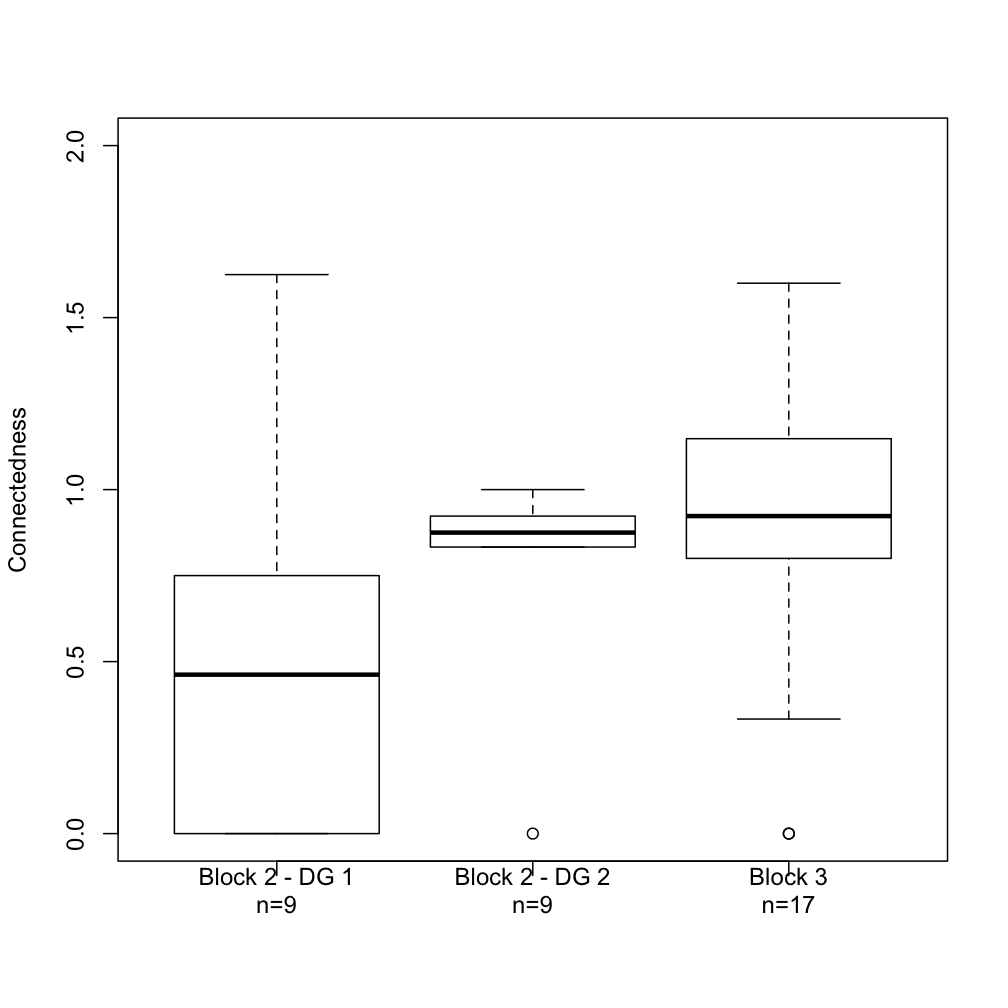
\includegraphics[height=3in]{img/Evaluierung/connectednessOverview.png}
	\caption{Connectedness in den Evaluierungsblöcken 2 und 3}
	\label{fig:img_Evaluierung_connectednessOverview}
\end{figure} 

Zu prüfen ist, ob die Connectedness in jenem Evaluierungs-Blöcken bzw. -Durchgängen, in denen die alternative Funktionalität zur Verbindungs-Herstellung verfügbar war, signifikant höher ist, als in jenen, in denen dies nicht der Fall war. Berechnet wird die Signifikanz zwischen den Ergebnissen der beiden Durchgänge von Block 2 ($conn_{2-1}$ -- $M=0.480, SD=0.544$ -- und $conn_{2-2}$ -- $M=0.804, SD=0.308$) sowie zwischen den Ergebnissen des ersten Durchgangs von Block 2 und den Ergebnissen von Block 3 ($conn_{3}$ -- $M=0.876, SD=0.435$). Im zweiten Fall ist zu beachten, dass die Aufgabenstellung nicht identisch war und diese Einfluss auf die Connectedness des Modells haben kann. Aufgrund der bestätigten Nicht-Normalverteilung der Stichprobe $conn_{2-2}$ (Sharpiro-Wilk-Test: $W_{2-1}=0.854, p_{2-1}=0.0823$, $W_{2-2}=0.586, p_{2-2}<0.005$, $W_{3}=0.913, p_{3}=0.114$) kommt zur Prüfung der Signifikanz der t-Test nicht in Frage, es wird der Wilcoxon-Test herangezogen.

Der einseitige Wilcoxon-Test für gepaarte Stichproben ergibt für $conn_{2-1}$ und $conn_{2-2}$ eine signifikant höhere Connectedness ($V=5, p=0.0400$) in der zweiten Stichprobe (jene mit Einsatz der alternativen Funktionalität der Verbindungsherstellung) als in der erste Stichprobe (ohne diese Funktionalität). 

Für $conn_{2-1}$ und $conn_{3}$ ergibt der einseitige Wilcoxon-Test für ungepaarte Stichproben ein ähnliches Ergebnis -- auch hier ist im der zweiten Stichprobe bei Einsatz der alternativen Funktionalität zur Verbiundungsherstellung eine signifikant höhere Connectedness festzustellen ($W=39, p=0.0227$).

Für $conn_{2-2}$ und $conn_{3}$ zeigt der zweiseitige Wilcoxon-Test für ungepaarte Stichproben dahingegen keine signifikant unterschiedliche Connectedness ($W=64.5, p=0.535$) für den zweitgenannten Block -- in diesem Fall kam in beiden Stichproben die alternative Möglichkeit zur Herstellung von Verbindungen zum Einsatz.

\subsubsection{Diskussion} % (fold)

Aufgrund der Ergebnisse der berechneten Signifikanztests ist die Hypothese anzunehmen. Mit der Einführung der alternativen Möglichkeit zur Herstellung von Verbindungen war in den einzelnen Anwendungen des Werkzeugs eine Zunahme der Verwendung von Verbindern zu beobachten. Während die Benutzer bei der ursprünglichen Funktion zur Herstellung von Verbindungen zum Großteil auf diese verzichteten (auch bereits in Evaluierungsblock 1), wurden Verbinder unabhängig von der Aufgabenstellung mit der Einführung der alternativen Funktionalität verstärkt eingesetzt.

Die Connectedness eignet sich als Parameter zur vergleichenden Beurteilung des Ausmaßes der Verwendung von Verbindern, da durch die Einbeziehung der Größe des Modells (repräsentiert durch die Anzahl der verwendeten Modellelemente) in die Berechnung den Wert für unterschiedliche Modelle vergleichbar macht. 

Einfluss auf die Höhe der Connectedness hat aber die Aufgabenstellung, die zur Bildung des Modells führt. Unterschiedliche Modellierungsaufgaben führen zu unterschiedlichen Modell-Topologien, die sich wiederum in der Anzahl der verwendeten Verbinder auswirkt. Die Concept-Mapping-Aufgabe, die $conn_{3}$ zugrunde liegt, führt eher zu stärker verbundenen Modellen führt als eher zur ablauforientierten Modellen führende Arbeitsabstimmungs-Aufgabe, auf der $conn_{2-2}$ basiert. Während bei Concept Mapping beliebige Konzepte in Beziehung stehen können, stehen Elemente bei ablauf-orientierten Modellen vor allem mit ihren kausalen Vorgängern und Nachfolgern in Beziehung, was die Anzahl der Verbinder einschränkt.

Dies ist am Ergebnis des Wilcoxon-Tests für $conn_{2-2}$ und $conn_{3}$ allerdings nicht zu erkennen -- in beiden Fällen stand die alternative Möglichkeit zur Verbindungsherstellung zur Verfügung. $conn_{3}$ unterscheidet sich nicht signifikant von $conn_{2-2}$. Die überarbeitete Möglichkeit zur Herstellung von Verbindern scheint die Auswirkung der unterschiedlichen Aufgabenstellung zu übertreffen.

Das Resultat der durgeführten Wilcoxon-Tests zwischen $conn_{2-1}$ und $conn_{2-2}$, $conn_{2-1}$ und $conn_{3}$ sowie $conn_{2-2}$ und $conn_{3}$ spricht für die Annahme der Hypothese \ref{hyp:verbinder}. Zu berücksichtigen ist hier jedoch die geringe Stichprobengröße, die die Aussagekraft des Ergebnisses schmälert.

\subsubsection{Ergebnis} % (fold)

Die Auswertung zeigt eine signifikant höhere Verwendung von Verbindern bei Verfügbarkeit der alternativen Funktionalität zur Verbindungs-Herstellung. Auch die Natur der Aufgabenstellung scheint hohen Einfluss auf die Verwendung von Verbindern zu haben (siehe dazu auch die Diskussion von Hypothese \ref{hyp:keine_verbinder} in Abschnitt \ref{sub:abbildung_von_zusammenhängen_ohne_verbinder}). \textbf{Hypothese \ref{hyp:verbinder} kann auf Basis der vorliegenden Daten bestätigt werden.}

% subsection herstellung_von_verbindern (end)

\subsection{Verwendung des Löschtokens} % (fold)
\label{sub:verwendung_des_löschtokens}

In diesem Abschnitt werden die Ergebnisse der Überprüfung der Hypothese \ref{hyp:radierer} („Das Löschtoken ermöglicht intuitives Löschen von Modellelementen.“) vorgestellt. Die Auswertung basiert auf den Ergebnissen der Modellierungsblöcke 2, 3, 4 und 5, wobei zwischen Evaluierungsblöcken 3 und 4 die Funktionaliät und Verwendungsweise des Tokens überarbeitet wurde.

\subsubsection{Auswertung} % (fold)

Zur Auswertung wurde erhoben, in welchem Ausmaß das Löschtoken zum Entfernen unerwünschter Verbinder im Gegensatz zur alternativen Möglichkeit -- dem Einsatz der Wiederherstellungsfunktion -- verwendet wurde. Zusätzlich wurde erhoben, in wie vielen Fällen die Verwendung des Löschtokens scheiterte, weil die Benutzer dessen Einsatzmöglichkeit inkorrekt interpretierten. Tabelle \ref{tab:fehlinterpretationen} zeigt diese Daten für die Evaluierungsblöcke 2 bis 5.

\begin{table}[htbp]
	\centering
	\caption{Verwendung des Löschtokens}
\begin{tabular}{| c || c || c | c | c | c |}
  \hline
   EB    & Anw. & $Lösch_{ges}$ & $Lösch_{Token}$ & $FI_{Token}$ & $Lösch_{WH}$ \\ \hline
   2     & 18 & 55 & 11 & 10 & 44 \\ 
   3     & 18 & 68 &  8 &  7 & 60 \\ 
   4     & 10 & 35 & 20 &  0 & 15 \\ 
   5     & 11 & 95 & 83 &  0 & 12 \\ \hline
   Ges.  & 57 & 253 & 122 & 17 & 131 \\ \hline
\end{tabular} \\
\footnotesize EB \ldots Evaluierungsblock, $Lösch_{ges}$ \ldots Gesamtanzahl der Löschvorgänge, $Lösch_{Token}$ \ldots Löschvorgänge mit Löschtoken, $FI_{Token}$ \ldots Fehlinterpretationen bei der Verwendung des Löschtokens, $Lösch_{WH}$ \ldots Löschvorgänge mit Wiederherstellungsfunktion
	\label{tab:fehlinterpretationen}
\end{table}

Die Fehlintepretation der Verwendung des Löschtokens kann durch die nähere Betrachtung mittels der durchgeführten Interaktionsanalyse exakter bestimmt werden. Ausgewählt wurden hier Beispiele aus den Modellierungsblöcken 2 und 3. Die gesammelten Transkripte sind in den in Anhang \ref{cha:daten_der_empirischen_untersuchung} genannten Quellen verfügbar.

In der ersten hier angeführten Szene versuchen die Teilnehmer, die Beschriftung eines Blocks mit dem Löschtoken auszuradieren. Dies scheitert, da das Löschtoken als Zustandsschalter fungiert und das eigentliche Löschen separat ausgelöst werden muss. Außerdem wirkt das Löschtoken nur auf Verbindungen.

\begin{transkript}
	\emph{Die Teilnehmer möchten einen Block umbenennen.}\\
	\textbf{A:} Wie haben wir jetzt gesagt \emph{(markiert den roten Baustein)} keine Modellierungsvorgabe \emph{(gibt Bezeichnung ein)}\\
	\emph{System übernimmt die neue Beschriftung für den Baustein nicht.}\\
	\textbf{A:} Wo wurde das hingeschrieben? \emph{(Pause)} Radiergummi? Glaubst du kann man das wegradieren?\\
	\textbf{B:} Probiere es aus.\\
	\textbf{\emph{A legt Radiergummi zum Block mit der Absicht die Beschriftung zu löschen}}\\
	\textbf{B:} Nein! Du löscht alles. Hör auf! \\
	\textbf{A:} Ok wie war das zuerst? Lassen wir das mal weg. \emph{(legt Baustein zur Seite)}\\
	\emph{A legt den Block zur Seite.} 
\end{transkript}

Ein ähnliches Missverständnis zeigt sich auch in dem im folgenden angegebenen Situation. Hier sollte eine Verbindung gelöscht werden, das Löschtoken wurde jedoch wiederum nicht als Zustandsschalter, sondern für den Vorgang des Löschens selbst verwendet.

\begin{transkript}
	\emph{TLN A und B stellen jeweils ihren Marker zu den Blöcken, die verbunden werden sollen. Dabei wird eine gerichtete Verbindung erstellt.}\\
	\textbf{C:} Jetzt haben wir aber einen Pfeil gebastelt.\\
	\textbf{B:} Ja stimmt. Interessant.\\
	\textbf{A:} Wie war das mit dem Radiergummi. \emph{(nimmt Radiergummi und legt ihn auf die Verbindung)}\\
	\textbf{B:} Nein\\
	\textbf{C:} Nein, mit dem Glas! Du löscht alles!\\
	\textbf{A:} Nein nur die Verbindung. \textbf{\emph{(Macht Radierbewegungen auf der Verbindung)}}\\
	\textbf{C:} Ich glaube dass wir das Glas nehmen müssen.\\
	\emph{A schiebt die Blöcke zwischen denen die Verbindung gelöscht werden soll zusammen.}\\
	\textbf{A:} Da es funktioniert. \emph{(schiebt die Blöcke weiter auseinander und bemerkt dass die Verbindung nicht gelöscht wurde)} Nein.\\
	\textbf{B:} Ich glaube der Radiergummi vernichtet alles.\\
	\textbf{A:} Nein der Radiergummi vernichtet nur Verbindungen. Nur welche? \emph{(schiebt beide Blöcke wieder zusammen – nimmt Radiergummi weg und schiebt Blöcke in die Ausgangsposition)}
\end{transkript}

In der folgenden Szene zeigen sich wiederum die Fehlinterpretationen der am Beginn angeführten Interaktion. Wieder wird das Token zum Radieren verwendet, Zielobjekt ist in diesem Fall die Beschriftung einer Verbindung.

\begin{transkript}
	\emph{Es wird eine falsche Beschriftung eingefügt. Die Teilnehmer wollen diese löschen, verwenden den Radiergummi allerdings falsch.}\\
	\textbf{B:} Aber irgendwie steht jetzt Ereignisse nicht bei dem Ding \emph{(zeigt auf gelben Block)} sondern dort \emph{(zeigt auf beschriftete Verbindung)}.\\
	\emph{A verrückt den gelben Block ein wenig.}\\
	\textbf{B:} Normal ist das nicht oder?\\
	\textbf{C:} Nein.\\
	\emph{A nimmt den Radiergummi.}\\
	\textbf{A:} Ich glaube das. \emph{(setzt den Radiergummi auf die Arbeitsfläche)}\\
	\textbf{C:} Aber nicht alles!\\
	\emph{A nimmt Radiergummi wieder weg. System erstellt eine Verbindung zwischen zwei roten Blöcken. Teilnehmer lachen. \textbf{A legt Radiergummi auf die erstellte Verbindung, und nimmt ihn wieder weg.} A nimmt die beiden verbundenen Blöcke und verschiebt sie.}\\
	\textbf{A:} Vielleicht so. \emph{(führt die Blöcke zusammen)}
\end{transkript}

In der folgenden Szene sind die Teilnehmer durch den Farbwechsel der Oberfläche beim Aufsetzen des Löschtokens (zur Indikation des Zustandswechsels) irritiert, da sie ebenfalls versuchen, das Token zum Radieren zu verwenden.

\begin{transkript}
	\emph{In der Szene erstellt das System einen ungewollten Verbinder, die Teilnehmer versuchen auf verschiedene Arten den Verbinder zu löschen.}\\
	\textbf{B:} Und wie kann ich die Verbindungen löschen?\\
	\textbf{B:} Warte einmal, da gibt es irgendwo das mit dem Radiergummi.\\
	\textbf{A:} murmelt zustimmend \\
	\emph{\textbf{B nimmt den Radiergummi und platziert ihn direkt auf dem Verbinder}}\\
	\emph{Das System färbt den Tisch rot}\\
	\textbf{A:} Nein, warte. Da löscht du Alles!\\
	\emph{\textbf{B verschiebt den Radiergummi auf dem Tisch, hebt ihn an und platziert ihn direkt auf einem Block.}}\\
	\emph{Sobald der Radiergummi von der Oberfläche auf den Block gelegt wurde, entfernt das System die rote Färbung.}\\
	\textbf{A:} Ich glaube da löscht du Alles.\\
	\emph{B legt den Radiergummi an mehreren Stellen trotz der Warnung von TN A auf die Oberfläche}\\
	\textbf{B:} Nein, es will eh nicht.\\
\end{transkript}

Die nachstehende Interaktion zeigt wiederum die in den anderen Szenen bereits beschriebene Fehlinterpretation in der Verwendung des Löschtokens. Zusätzlich verwirrt eine Fehlfunktion des Werkzeugs, das anstelle eines Löschvorgangs einen Verbinder hinzufügt.

\begin{transkript}
	\emph{C versucht die Benennung eines Verbinders mittels Radiergummi zu entfernen.}\\
	\textbf{B:} Aber irgendwie steht jetzt Ereignisse nicht bei dem Ding \emph{(deutet auf einen Block)} sondern dort \emph{(deutet auf einen Verbinder)}. Das wollen wir nicht oder?\\
	\textbf{A:} Nein.\\
	\textbf{C:} Ich glaube das. \emph{\textbf{(nimmt den Radiergummi und legt ihn auf den Verbinder den die Teilnehmer entfernen wollen.)}}\\
	\textbf{A:} Aber nicht alles.\\
	\emph{C entfernt den Radiergummi wieder von der Modellierungsoberfläche. In diesem Moment erstellt das System durch Fehlerkennungen automatisch einen neuen Verbinder. C versucht den neuen Verbinder mittels Radiergummi zu entfernen.}\\
	\textbf{A:} Oh Gott.\\
	\textbf{C:} Vielleicht so \emph{(schiebt die beiden betroffenen Blöcke zusammen)}, nein.\\
	\textbf{B:} Nein.\\
	\textbf{A:} Oh Gott oh Gott oh Gott.\\
	\textbf{B:} Gehen wir einen Prozessschritt zurück.\\
	\textbf{C:} Genau.\\
\end{transkript}

In der letzten hier angeführten Szene interagieren die Teilnehmer beinahe wie im Interaktionsdesign ursprünglich intendiert mit dem System. Sie scheitern letztendlich trotzdem und greifen zu alternativen Möglichkeit der Fehlerkorrektur, der Wiederherstellungsfunktion.

\begin{transkript}
	\emph{Teilnehmer versuchen mit dem Radiergummi und nur einem anderen Marker einen Verbinder zu entfernen.}\\
	\textbf{B:} Können wir die nicht so auch einfach löschen?\\
	\textbf{C:} Ja mit dem Radiergummi.\\
	\textbf{B:} Muss ich den jetzt zuerst so \emph{(Hält den Radiergummi zur Kamera)} hinhalten?\\
	\textbf{A:} Nein, ich glaube, \textbf{den musst du einfach da \emph{(zeigt auf den Verbinder)} drauf legen.}\\
	\emph{B legt den Radiergummi auf den vom System automatisch erstellten Verbinder.}\\
	\textbf{A:} Und jetzt muss man \emph{(legt ein Markierungtoken auf den Verbinder)} Nein.\\
	\emph{Der Verbinder lässt sich auf diese Art nicht löschen und die Teilnehmer entscheiden sich den Fehler mittels der Wiederherstellungsfunktion zu beseitigen.}
\end{transkript}

\subsubsection{Diskussion} % (fold)

In der quantitativen Auswertung ist klar zu erkennen, dass die ursprüngliche Implementierung der Löschfunktion, in der das Löschtoken als Zustandsumschalter fungierte, von den Benutzern kaum verwendet wurde und in jenen Fällen, in dem sie zum Einsatz kam, falsch interpretiert wurde, was letztendlich zum Scheitern des Löschvorgangs führte. Beginnend mit Block 4 wurde die Löschfunktion in einer vollständig erneuerten Implementierung eingesetzt, in der das Löschtoken tatsächlich zum Löschen einer Verbindung verwendet werden konnte. Damit wurde der vorherrschenden Interpretation der Funktionalität durch die Benutzer Rechnung getragen, was sich dadurch äußert, dass die Anzahl der Fehlinterpretationen auf 0 sank und das Löschtoken in weitaus höherem Ausmaß als die Wiederherstellungsfunktion zur Fehlerkorrektur verwendet wurde.

Bei der Betrachtung der Hypothese muss also zwischen der ursprünglichen Implementierung und deren neuen Umsetzung unterschieden werden. Für die ursprüngliche Implementierung kann die Hypothese nicht bestätigt werden, das Werkzeug war in der vorliegenden Form für die Benutzer nicht verständlich. In der Neuimplementierung wurden die ursprünglichen Fehlinterpretationen berücksichtigt und das Werkzeug zu modifiziert, dass es entsprechend der beobachteten Benutzerinterpretation verwendet werden konnte. In dieser Variante sprechen die erhobenen Daten für eine Bestätigung der Hypothese.

\subsubsection{Ergebnis} % (fold)

\textbf{Hypothese \ref{hyp:radierer} muss für die ursprüngliche Umsetzung der Löschfunktion abgelehnt werden, kann aber für die neu konzipierte und implementierte Variante bestätigt werden.} In der ursprünglichen Umsetzung war die Verwendung des Werkzeugs für die Benutzer nicht verständlich, die eigentlich aufwändigere Alternativfunktion zur Fehlerkorrektur wurde außerdem weitaus häufiger verwendet. Nach der Neukonzeption kam es zu keinen Fehlinterpretationen mehr, das Löschtoken wurde außerdem in weitaus höherem Ausmaß verwendet.

% subsection verwendung_des_löschtokens (end)
% section ergebnisse (end)

\section{Zusammenfassung}
\label{sec:t_zusammenfassung}

In diesem Kapitel wurde die Evaluierung der Verwendbarkeit des Werkzeugs beschrieben. Die hier formulierten Hypothesen beschäftigen sich dementsprechend mit den grundlegenden Funktionen des Werkzeugs und den Interaktionsmöglichkeiten der Benutzer mit diesen. Nicht Gegenstand dieses Kapitels waren die im Kontext der Durchführung von „Articulation Work“ erstellten Modelle (siehe Kapitel \ref{cha:eval_aw}) sowie die Auswirkungen der Durchführung in der „Production Work“ (siehe Kapitel \ref{cha:eval_aw}).

In diesem Kapitel wurden sechs Hypothesen zur Werkzeugbenutzung getestet, die unmittelbar aus den Anforderungen an das Werkzeug (siehe \ref{cha:anforderungen}) abgeleitet waren. Zwei weitere Hypothesen zur Werkzeugverwendung wurden im Verlauf der ersten Evaluierungsblöcke explorativ gebildet und in den späteren Evaluierungsblöcken getestet. Die sechs aus den Anforderungen abgeleiteten Hypothesen bilden im Wesentlichen die Kernfunktionen des bzw. Interaktionsmöglichkeiten mit dem Werkzeug ab. Durch die Prüfung dieser Hypothesen wird so das gesamte Werkzeug einer Überprüfung hinsichtlich dessen praktischer Verwendbarkeit unterzogen.

Hypothese \ref{hyp:diagmodelle} („Repräsentation diagrammatischer Modelle“) bildet den grundlegenden Anspruch des Werkzeugs ab, die Abbildung von diagrammatischen Modellen zu ermöglichen. Diese werden als Repräsentation für externalisierte mentale Modelle verwendet und bilden so die Grundlage für die Durchführung von expliziter „Articulation Work“. Diese Hypothese konnte im Rahmen der Untersuchung bestätigt werden. Die Abbildung von Konzepten und Beziehungen zwischen diesen wurde in allen vorliegenden Modellen erfolgreich umgesetzt, wenngleich die Modellierung von expliziten Verbindungen in den ersten beiden Evaluierungsblöcken aufgrund von technischen Unzulänglichkeiten nicht durchgeführt wurde.

Hypothese \ref{hyp:kollaborativ} („Kooperatives Arbeiten“) prüft, ob die kooperative Verwendung des Werkzeugs möglich ist. Für die Durchführugn von „Articulation Work“ ist der kooperative Einsatz notwendig, da nur so die dabei ablaufenden synchronen Abstimmungsprozesse ermöglicht bzw. unterstützt werden können. Die Hypothese konnte in der Untersuchung bestätigt werden. Der Zeitanteil an der Modellbildung ist für Anwendungen mit zwei Teilnehmern weitgehend gleichverteilt, beide Teilnehmer beteiligen sich also an der Modellierung. Bei mehr als zwei Anwendern ist die Gleichverteilung nicht mehr gegeben, die Teilnehmer haben dennoch durchwegs (unabhängig von der Anzahl der Teilnehmer bei einer Anwendung) den Eindruck sich einbringen zu können und gut zusammenarbeiten zu können.

Hypothese \ref{hyp:kontexte} („Einsetzbarkeit in unterschiedlichen Kontexten“) legt den Anspruch an das Werkzeug fest, das dessen Anwendung unabhängig von der konkreten Anwendungsdomäne möglich ist. Wesentlich ist hierbei, das das Werkzeug von Teilnehmer mit unterschiedlichen beruflich bzw. Ausbildungs-Hintergründen gleich gut verwendet werden kann und dass die Modellbildung durch das Werkzeug nicht spezifisch für bestimmte Aufgabenstellungen erschwert wird. Die Hypothese konnte im Rahmen der Untersuchung bestätigt werden. Die Untersuchung der Korrelation zwischen Modellgröße und Modellierungsdauer zeigt unabhängig vom Anwendungskontext eine stark positive Korrelation, was darauf hinweist, das der Aufwand zur Modellerstellung unabhängig von Aufgabenstellung und Anwendungskontext relativ stabil bleibt. Auch die Rückmeldungen der Teilnehmer mit unterschiedlichen beruflichen Hintergründen sind im Wesentlichen identisch, so dass das Werkzeug unabhängig vom Anwendungskontext immer ähnliche Wirkungen auf die Modellbildung zu haben scheint. 

Hypothese \ref{hyp:wiederherstellung} („Wiederherstellung vergangener Modellzustände“) prüft, ob die Bereitschaft zur Erstellung unterschiedlicher Modellvarianten im Verlauf der Modellbildung durch die Möglichkeit zur Wiederherstellung vergangener Modellzustände gefördert wird. Diese Hypothese kann auf Basis der Untersuchung nicht bestätigt werden. Die Wiederherstellungsfunktion wird nur in unter 10\% der untersuchten Anwendungen zur Verfolgung alternativer Modellierungswege genutzt. Die Funktion wird außerdem von den Anwendern bei der Frage nach den als nützlich wahrgenommene Funktionen in keinem der betrachten Fälle genannt, so dass davon ausgegangen werden muss, das sie nicht als relevant für die Durchführung der Modellbildung erachtet wird.

Hypothese \ref{hyp:behinderung} („Nicht-Behinderung“) geht auf die Gesamtwirkung des Werkzeugs bei der Modellbildung ein und untersucht, ob diese durch das Werkzeug behindert wird. Im Wesentlichen sind Bedienungsprobleme und technische Fehlfunktionen des Werkzeugs zu betrachten, die einen negativen Effekt auf die Ausführung der eigentlichen Aufgabe haben können. Die Hypothese konnte im Rahmen der Untersuchung nicht bestätigt werden. Bei der Benutzung des Werkzeugs traten vor allem in den ersten Evaluierungsblöcken Fehlfunktionen auf, die die Modellbildung massiv behinderten oder teilweise verhinderten. Durch Stabilisierung und Überarbeitung der technischen Plattform konnten diese Fehlfunktionen zwar minimiert werden, insgesamt können die Verbesserungen die gemessenen Werte nicht soweit verbessern, dass die Hypothese statistisch signifikant bestätigt werden könnte. Diese erhobenen Aspekte sind auch durch die überwiegend positive Benutzereinschätzung des Werkzeuges nicht als kompensiert anzusehen.

Hypothese \ref{hyp:gewöhnung} („Gewöhnung an das Werkzeug“) prüft, ob die wiederholte Verwendung des Werkzeugs dessen Bedienbarkeit durch die Benutzer verbessert. Betrachtet wurde hier einerseits die Modellierungsdauer im Verhältnis zur Modellgröße, was ein Maß für die Geschwindigkeit der Modellierung darstellt. Andererseits wurde die Anzahl der Fehlbedienungen des Werkzeugs betrachtet, die bei besserer Bedienbarkeit in wiederholten Anwendungen geringer ausfallen sollte. Die Hypothese kann auf Basis der vorliegenden Daten nur teilweise bestätigt werden. Während kein signifikanter Beschleunigungseffekt bei wiederholter Verwendung des Werkzeugs festgestellt werden konnte, war eine signifikante Verringerung der Anzahl der Fehlbedienungen des Werkzeugs bei wiederholtem Einsatz feststellbar.

Hypothese \ref{hyp:keine_verbinder} („Herstellung von Verbindern“) wurde explorativ aus Beobachtungen in den Evaluierungsblöcken 2 und 3 abgeleitet. In diesen Blöcken stieg die Verwendung von Verbindern im Modell sprunghaft an. Geprüft wurde nun, ob dies -- wie vermutet wurde -- auf die überarbeiteten und erweiterten Möglichkeiten zur Herstellung von Verbindern im Modell zurückzuführen war. Die Hypothese konnte in der Untersuchung bestätigt werden. Die Auswertung zeigt eine signifikant höhere Verwendung von Verbindern bei Verfügbarkeit der überarbeiteten Funktionalität zur Verbindungs-Herstellung. Allerdings scheint auch die Natur der Aufgabenstellung hohen Einfluss auf die Verwendung von Verbindern zu haben. Diese Vermutung wurde in Hypothese \ref{hyp:keine_verbinder} nochmals aufgegriffen und dort genauer untersucht (siehe dazu  Abschnitt \ref{sub:abbildung_von_zusammenhängen_ohne_verbinder}).

Hypothese \ref{hyp:radierer} („Verwendung des Löschtokens“) betrachtet ebenfalls eine Funktionalität des Werkzeugs, die auf Basis von Beobachtungen der Benutzerinteraktionen überarbeitet wurde. Die Funktion zur Entfernung von Verbindern wurde in den ersten Evaluierungblöcken kaum verwendet und zeigte im Falle der Verwendung hohes Potential für Missverständnisse hinsichtlich der Art der Benutzung. Die zur Verwendung notwendigen Interaktionsabläufe wurden daraufhin an die offensichtlich vorherrschende Interpretation der Benutzter, wie das entsprechende Werkzeug zu verwenden wäre, angepasst. Untersucht wurde nun, ob diese Anpassung die Entfernung von Elementen aus dem Modell erleicherte bzw. intuitiv gestaltete. Die Hypothese konnte für die überarbeitete Variante des Löschtokens bestätigt werden. In der ursprünglichen Umsetzung war die Verwendung des Werkzeugs für die Benutzer nicht verständlich, die eigentlich aufwändigere Alternativfunktion zur Fehlerkorrektur mittels der Wiederherstellungsfunktion wurde außerdem weitaus häufiger verwendet. Nach der Neukonzeption kam es zu keinen Fehlinterpretationen mehr, das Löschtoken wurde außerdem in weitaus höherem Ausmaß verwendet.

Insgesamt zeigt sich, dass das Werkzeug in der vorliegenden Form weitgehend verständlich zu sein scheint und als nützlich sowie zum Teil benutzbar wahrgenommen wird. Das Werkzeug erfüllt die Grundanforderungen hinsichtlich der Abbildbarkeit diagrammatischer Modelle und der Ermöglichung kooperativen Arbeitens. Die Einsetzbarkeit in beliebigen Kontexten scheint gegeben zu sein, wobei aufgrund von technischen Instabilitäten die Verwendbarkeit vor allem in den frühen Phasen der Evaluierung eingeschränkt war. Jene Hypothesen, die auf die Verwendung spezifischer Funktionalitäten eingehen, zeigen eine gute Verständlichkeit und hohes Ausmaß an Verwendung der Basisfunktionalitäten der Modellierung (etwa Platzierung und Benennung von Blöcken, Herstellung von Verbindern, Löschen von Verbindern), offenbaren aber Schwächen in der Verständlichkeit und Akzeptanz der komplexeren Funktionen, wie etwa der Wiederherstellungsunterstützung für gespeicherte Modellzustände. Zusammenfassend scheint das Werkzeug den grundlegenden Anforderungen also gerecht zu werden, bietet aber Raum für Verbesserungen hinsichtlich der Verwendung der komplexeren Funktionen und der technischen Stabilität. Im folgenden Kapitel wird nun auf die Verwendung des Werkzeugs zur kooperativen Abbildung von Modellen eingegangen. 

% chapter eval_tui (end) 